%% Copernicus Publications Manuscript Preparation Template for LaTeX Submissions
%% ---------------------------------
%% This template should be used for the following class files: copernicus.cls, copernicus2.cls, copernicus_discussions.cls
%% The class files, the Copernicus LaTeX Manual with detailed explanations regarding the comments
%% and some style files are bundled in the Copernicus Latex Package which can be downloaded from the different journal webpages.
%% For further assistance please contact the Publication Production Office (production@copernicus.org).
%% http://publications.copernicus.org


%% Differing commands regarding the specific class files are highlighted.


%% copernicus.cls
%\documentclass[gmd]{copernicus}

%% copernicus2.cls
%\documentclass[gmd]{copernicus2}

%% copernicus_discussions.cls
\documentclass[gmdd, hvmath, online]{copernicus_discussions}

\usepackage{amsmath}
\usepackage{graphicx}
\usepackage{multicol}
\usepackage{natbib}
\usepackage{wrapfig}
\usepackage{hyperref}
\usepackage{tabularx}
\usepackage{setspace}
\usepackage{comment}
\usepackage{color}
\usepackage{float}
\usepackage{rotfloat}
\usepackage{rotating}

\newcommand\BibTeX{{\rmfamily B\kern-.05em \textsc{i\kern-.025em b}\kern-.08em
T\kern-.1667em\lower.7ex\hbox{E}\kern-.125emX}}

\usepackage{newfloat}
\DeclareFloatingEnvironment[fileext=frm,placement={!ht},name=Algorithm]{algorithm}
\captionsetup[algorithm]{labelfont=bf}

% Custom commands
\newcommand{\vb}{\mathbf}
\newcommand{\vg}{\boldsymbol}
\newcommand{\mat}{\mathsf}
\newcommand{\diff}[2]{\frac{d #1}{d #2}}
\newcommand{\diffsq}[2]{\frac{d^2 #1}{{d #2}^2}}
\newcommand{\pdiff}[2]{\frac{\partial #1}{\partial #2}}
\newcommand{\pdiffsq}[2]{\frac{\partial^2 #1}{{\partial #2}^2}}


\begin{document}

\linenumbers

\title{TempestExtremes:  A Framework for Scale-Insensitive Pointwise Feature Tracking on Unstructured Grids}

\author{Paul A. Ullrich and Colin Zarzycki}

\affil{Paul A. Ullrich, Department of Land, Air and Water Resources, University of California, Davis, One Shields Ave., Davis, CA 95616.  Email: paullrich@ucdavis.edu}

\runningtitle{A Framework for Scale-Insensitive Pointwise Feature Tracking ...}

\runningauthor{P.~A.~Ullrich and C.~Zarzycki}

\correspondence{Paul A. Ullrich\\ (paullrich@ucdavis.edu)}



\received{}
\pubdiscuss{} %% only important for two-stage journals
\revised{}
\accepted{}
\published{}

%% These dates will be inserted by the Publication Production Office during the typesetting process.


\firstpage{1}

\maketitle  %% Please note that for the copernicus2.cls this command needs to be inserted after \abstract{TEXT}



\begin{abstract}
Automated pointwise feature tracking is an algorithmic technique for identification and tracking of meteorological features such as extratropical cyclones, tropical cyclones and tropical easterly waves, and has emerged as an important and desirable data processing capability in climate science.  Software tools for feature tracking -- typically referred to as ``trackers'' -- have been employed throughout the literature to answer pressing scientific questions on anticipated changes in atmospheric features under climate change.  This paper describes a new open-source software framework for pointwise feature tracking that is applicable to a wide array of climate datasets using either structured or unstructured grids.  To enable support for a wide array of detection schemes, a suite of algorithmic kernels have been developed that capture the core functionality of algorithmic tracking routines from throughout the literature.  A review of efforts related to pointwise feature tracking from the past three decades is included.  Selected results using both reanalysis datasets and unstructured grid simulations are provided.
\end{abstract}


%% only used for copernicus2.cls
%\abstract{
% TEXT
% \keywords{TEXT}}



\introduction  %% \introduction[modified heading if necessary]
%TEXT

Automated pointwise feature tracking has emerged as an important and desirable data processing capability in climate science.  Software tools for feature tracking -- typically referred to as ``trackers'' -- have been employed throughout the literature to answer pressing scientific questions on anticipated changes in atmospheric features under climate change.  Exploration of the literature on trackers exposes a vast breadth of potential techniques (see Appendices \ref{sec:ExtratropicalCycloneAlgorithms}, \ref{sec:TropicalCycloneAlgorithms} and \ref{sec:TropicalEasterlyWaveAlgorithms}) that have been applied to climate datasets with varied spatial resolution and temporal frequency.  Nonetheless, the definition of an optimal objective criteria for key atmospheric features has eluded development, and ambiguity in the formal definition of these features suggests that there may be no singular criteria capable of both perfect detection and zero false positive rate.  Further, as observed by \cite{walsh2007objectively} for tropical cyclones and \cite{neu2013imilast} for extratropical cyclones, feature tracking schemes can produce wildly varying results depending on the specific choice of threshold variables and values.  Consequently, we argue that conclusions drawn from these trackers should use an ensemble of detection thresholds and variables.  To this end, it is the goal of this paper to develop and present a unified framework that enables a variety of tracking procedures applicable across effectively arbitrary spatial resolution and temporal frequency.

Most algorithmic trackers of pointwise features (such as cyclones and eddies) share a common detection procedure:
\begin{itemize}
\item[1.] Identify an initial set of candidate points by searching for local extrema.  Local extrema can be further isolated, for instance, by requiring that the local extrema be sufficiently anomalous when contrasted with their neighbors.  For most cyclonic structures, either minima in the sea level pressure field or maxima in the absolute value of the relative vorticity are used.
\item[2.] Eliminate candidate points that do not satisfy a prescribed set of thresholds.  For instance, tropical cyclones typically require the presence of an upper-level warm core that is sufficiently near the sea level pressure minima that defines the storm center.
\item[3.] Connect candidate points together in time to generate feature paths, eliminating paths that are of insufficient length or do not meet additional criteria.
\end{itemize}  The procedure described above fits into a general framework known as MapReduce \citep{dean2008mapreduce}, which is a combination of a Map(), an embarrassingly parallel candidate identification procedure applied to individual time slices, and a Reduce(), which stitches candidates across time to build feature tracks.  A key advantage of employing this framework is that substantial work has been undertaken to understand optimal strategies for parallelization of MapReduce-type algorithms (e.g. \cite{Prabhat2012}) in order to mitigate bottlenecks associated with I/O and load balancing.  TempestExtremes currently implements a simple parallelization strategy via MPI, although future work on this issue is forthcoming.

The development of a framework for feature tracking that is robust across essentially arbitrary datasets requires some additional considerations.  In particular, we expect that our framework should:
\begin{itemize}
\item[] ...use great-circle arcs for all distance calculations.  This avoids issues associated with latitude-longitude distance that emerges near the poles.
\item[] ...support structured and unstructured grids.  This eliminates the need for post-processing of large native-grid output files and enables detection and characterization simultaneous with the model execution.
\item[] ...not contain hard-coded variable names, so as to ensure robust applicability across reanalysis datasets and applicability to a variety of problems.
\item[] ...allow for easy intercomparison of detection schemes by enabling detection criteria and thresholds that are compactly specified on the command line.
\end{itemize}  Well-known automated software trackers include Kevin Hodges' TRACK code \citep{hodges2015track} and the Geophysical Fluid Dynamics Laboratory (GFDL) TSTORMS package \citep{TSTORMS} {\color{red}Others?}.  Both of these software packages have been used extensively throughout the literature for studies examining pointwise features in the atmosphere, but do not completely satisfy our four requirements above.

Although the actual procedures used for feature tracking vary throughout the literature, a review of this material reveals several core algorithms (kernels) must be exposed to the user.  Based on our analysis, the most commonly employed kernels are as follows:
\begin{itemize}
\item Computation of anomalies in a data field from a spatially averaged mean.
\item Identification of local extrema in a given 2D data field (for instance, sea level pressure minima).
\item Determination of whether a closed contour exists in a data field around a particular point.
\item Determination of whether, in the neighborhood of a particular point, a data field satisfies a given threshold.
\item Stitching of candidates from sequential time slices to build feature tracks.
\end{itemize}  It is desirable that any generalization these kernels is insensitive to the spatial resolution of the input data; that is, criteria that require averaging or searching over a discrete number of grid points around each candidate (which is common throughout the early tracking literature) is incompatible with scale insensitivity since detection would be dependent on the spatial resolution of the data. Note that identification of local extrema is not a resolution-insensitive procedure, since the number of extrema will often scale with the number of spatial data points, and so initial identification is typically augmented with the more scale-insensitive closed contour criteria (see section \ref{sec:ClosedContour}).

The remainder of the paper is organized as follows:  Section \ref{sec:Kernels} describes the algorithms and kernels that have been implemented in the TempestExtremes software framework.  Selected examples of tropical cyclone, extratropical cyclone and tropical easterly wave detection are then provided in section \ref{sec:SelectedExamples}, followed by conclusions in section \ref{sec:Conclusions}.  The appendices provide a review of relevant literature on pointwise feature trackers of extratropical cyclones (appendix \ref{sec:ExtratropicalCycloneAlgorithms}), tropical cyclones (appendix \ref{sec:TropicalCycloneAlgorithms}) and tropical easterly waves (appendix \ref{sec:TropicalEasterlyWaveAlgorithms}).  A technical guide to the use of the TempestExtremes tools \texttt{DetectCyclonesUnstructured} and \texttt{StitchNodes} is provided in appendices \ref{sec:DetectCyclonesUnstructuredAppendix} and \ref{sec:StitchNodesAppendix}.

\subsection{Code and Data Availability}

The open-source software described in this manuscript has been released as part of the TempestExtremes software package, and is available for use under the Lesser GNU Public License (LGPL).  All software can be obtained from GitHub at:
\begin{center}
\texttt{https://github.com/ClimateGlobalChange/tempestextremes}
\end{center} 

%However, there is a growing need for scale-insensitive detection techniques and unstructured grid support that is not well met with existing schemes.  Consequently, it is the goal of this paper is to describe a tracking technique that can be applied on essentially any grid at any resolution, and provide insight into currently available algorithmic techniques underlying modern tracking algorithms.

%\section{Automated tracking}

%\subsection{Extratropical cyclones}


%\subsection{Tropical cyclones}

%Extratropical cyclone tracking techniques have been modified in order to support tropical cyclone tracking.  To eliminate ``false positives'' associated with extratropical cyclones and weak cyclonic depressions, many schemes require that the candidate be associated with a nearby warm core and be associated with a minimum threshold on surface winds for at least 1-3 days.  The definition of a ``warm core'' varies between modeling centers, including such options as air temperature anomaly on pressure surfaces \citep{Vitart1997,Zhao2009,Murakami2012}, geopotential thickness \citep{tsutsui1996simulated} and decay of vorticity with height \citep{Bengtsson2007,Strachan2013}.  Additional filtering of candidate storms over topography or within a specified latitudinal range may be required.  To better match observations, additional geographical, model or feature-dependent criteria may be applied \citep{camargo2002improving,Walsh2007,Murakami2010,Murakami2012}.  In \cite{broccoli1990existing}, tropical cyclone-like features were detected by seeking local minima (occupying one grid point due to the coarse model resolution) in the surface pressure field that accompanied a minimum surface wind speed of 17 m/s.  A tracking procedure was also developed using a minimum distance between detections that represented a maximum velocity of 50 km/hr for TCs.  Tracking in \cite{haarsma1993tropical} instead detected maxima in the 850mb relative vorticity (greater than $3.5 \times 10^{-5} \mbox{s}^{-1}$ accompanied by a weak warm core (using local temperature anomaly at 250mb, 500mb and 850mb) and required TCs to exist for a minimum of 3 days.  \cite{bengtsson1995hurricane} made use of thresholds on 850mb relative vorticity, maximum local velocity, temperature anomaly at 700, 500 and 300 hPa and required systems exist for at least 1.5 days.  \cite{tsutsui1996simulated} detects geopotential height minima at 1000mb and then imposes additional thresholds on 900mb relative vorticity, divergence, vertical pressure velocity, geopotential thickness and zonal wind velocity.  \cite{camargo2002improving} use the absolute value of relative vorticity for detection, then further employ thresholds on maximum wind speed, sea level pressure, temperature anomaly, mean wind speed and track length.

%A review of tropical cyclone detection algorithms can be found in Appendix \ref{sec:TropicalCycloneAlgorithms}.  

\section{TempestExtremes Algorithms and Kernels} \label{sec:Kernels}

This section describes the building blocks that have been utilized in constructing our detection and characterization framework.  As mentioned earlier, in order to avoid sensitivity of the detection scheme to grid resolution, great-circle-distance has been employed throughout.  In terms of regular latitude-longitude coordinates, great-circle-distance between points $(\lambda_1, \varphi_1)$ and $(\lambda_2, \varphi_2)$ is defined via the symmetric operation
\begin{equation}
r(\lambda_1, \varphi_1; \lambda_2, \varphi_2) = a \arccos \left( \sin \varphi_1 \sin \varphi_2 + \cos \varphi_1 \cos \varphi_2 \cos (\lambda_1 - \lambda_2) \right).
\end{equation}  Algorithmically, this calculation is implemented as \texttt{gcdist(p,q)} for given graph nodes \texttt{p} and \texttt{q}.

\subsection{Efficient neighbor search using $k$-d Trees}

Three-dimensional ($k=3$) $k$-d trees \citep{bentley1975multidimensional} are used throughout our detection code using the implementation of \cite{tsiombikas2015kdtree}.  Although $k$-d trees use 3D straight-line instance instead of great-circle-distance, we utilize the observation that straight-line and great-circle distance maintain the same ordering for points confined to the surface of the sphere.  In particular, we utilize three key functions made available by the $k$-d tree implementation:
\begin{itemize}
\item[] \texttt{K = build\_kd\_tree(P)} constructs a $k$-d tree \texttt{K} from a point set \texttt{P}.
\item[] \texttt{q = kd\_tree\_nearest\_neighbor(K, p)} locates the nearest neighbor \texttt{q} to point \texttt{p} using the $k$-d tree \texttt{K}.
\item[] \texttt{S = kd\_tree\_all\_neighbors(K, p, dist)} locates all points that are within a distance \texttt{dist} of a point \texttt{p} within the $k$-d tree \texttt{K}.
\end{itemize}

\noindent A key advantage of $k$-d trees is their relatively efficient $O(n \log n)$ construction time and $O(\log n)$ average time nearest neighbor search.

\subsection{Unstructured grid specification}

For purposes of determining connectivity of the unstructured grid, we require the specification of a graph such as the one depicted in Figure \ref{fig:unstructured_grid}.  The connectivity information is stored textually as an adjacency list via a variable-length comma-separated variable file.  The total number of nodes ($N$) is specified at the top of the file, followed by $N$ lines containing the longitude (lon), latitude (lat), associated area, number of adjacent nodes, and finally a 1-indexed list of all adjacent nodes, such as depicted below:
\ \\

\noindent \begin{tabular}{|p{\textwidth}|}
\hline \small \begin{verbatim}
<total number of nodes>
<lon>,<lat>,<area>,<# adj. nodes>,<first adj. node>,..,<last adj. node>
...
\end{verbatim} \\
\hline
\end{tabular}

\subsection{Computing a spatial averaged mean}

Many existing tracking algorithms use either a spatially-averaged mean field or an anomaly field computed against the spatially-averaged mean \citep{haarsma1993tropical,bengtsson1995hurricane}.  The mean operation (implemented in TempestExtremes as \texttt{\_MEAN()} in the variable specification) is computed on unstructured grids via graph search (see Algorithm \ref{alg:field_mean_value}).  Anomaly from the mean can then be computed in conjunction with the \texttt{\_DIFF} operator (see appendix \ref{sec:VariableSpecification}).

\subsection{Extrema detection}

For purposes of computational efficiency, candidate points are initially located by identifying local extrema in a given field (for instance SLP) via \texttt{find\_all\_minima} (Algorithm \ref{alg:find_all_minima}).  Candidates are then eliminated if they are ``too close'' to stronger extrema (Algorithm \ref{alg:merge_candidates_minima}) (e.g. \cite{pinto2005sensitivities}).  The initial search field is specified to TempestExtremes either via the \texttt{--searchbymin} or \texttt{--searchbymax} command line argument.  The merge distance used in \texttt{merge\_candidates\_minima} is specified via the \texttt{--mergedist} command line argument.

\subsection{Closed contour criteria} \label{sec:ClosedContour}

Although a first pass at candidate points may be made by looking for local extrema (comparing against all neighboring nodes), this criteria is not robust across model resolution.  That is, the distance between a node and its neighbors decreases proportional to the local grid spacing, and so does not definite ``physical'' criterion.  Consequently, we instead advocate for a \textit{closed contour criteria} to define candidate nodes.  Closed contours were first employed by \cite{bell198915}, who used a 30m 500 mb geopotential height contour to identify closed circulation centers.  Their approach used radial arms generated at 15$^\circ$ intervals over a great-circle-distance of 2$^\circ$ and required that geopotential heights rise by at least 30m along each arm.  Unfortunately, the use of radial arms to define the closed contour is again sensitive to model resolution, since it has the potential to only sample as many neighbors as radial arms employed.

Here we propose an alternative closed contour criteria that is largely insensitive to model resolution that uses graph search to ensure that all paths along the unstructured grid from an initial location \texttt{p0} lead to a sufficiently large decrease (or increase) in a given field \texttt{G}.  This criteria is illustrated in Figure \ref{fig:ClosedContour}, and is implemented in Algorithm \ref{alg:find_max_near} and \ref{alg:closed_contour_max} (for closed contours around local maxima).  The closed contour criteria is implemented in TempestExtremes via the command line argument \texttt{--closedcontourcmd}.  An analogous command line argument \texttt{--noclosedcontourcmd} is also provided, which has similar functionality but discards candidates that satisfy the closed contour criteria (this may be desirable, for instance, to identify cyclonic structures that do not have a warm core).

\subsection{Thresholding}

Additional threshold criteria may be applied at the Map() stage in order to further eliminate undesirable candidates.  For example, a common threshold criteria requires that a field \texttt{G} satisfy some minimum value within a distance \texttt{dist} of the candidate, as implemented in Algorithm \ref{alg:threshold_max}.

\subsection{Stitching}

The basic track stitching procedure (which represents the Reduce() stage in MapReduce) is implemented in Algorithm \ref{alg:stitch_nodes} using the output from the Map() procedure at each time level (stored in set array \texttt{P[1..T]}), a maximum great-circle-distance between nodes, \texttt{dist}, and a maximum gap size, \texttt{maxgap}.  Here, gap size refers to the maximum number of sequential non-detections that can occur before a path is considered terminated.  This argument is useful, for instance, for tracking tropical storms that temporarily weaken before strengthening into tropical cyclones.

For simplicity, $k$-d trees are constructed at each time level in order to maximize the efficiency of the search.  Each candidate pair (time, node) can only be used in one path, and so construction simply requires exhausting the list of available candidates.  Once paths have been constructed, additional criteria can be applied -- for instance, minimum path length or additional criteria based on minimum path length or minimum distance between the start and endpoints of the path (see Appendix \ref{sec:StitchNodesAppendix}).  Thresholds based on field values may also be applied, \textit{e.g.} sea level pressure must be below a particular value for at least 8 time steps of each track.

\section{Selected examples} \label{sec:SelectedExamples}

Several selected examples of the feature detection tool are now provided.  The first three examples use data from the NCEP Climate Forecast System Reanalysis (CFSR), available at 0.5 degree global resolution with 6-hourly output from 1979-present \citep{saha2010ncep}.  The remaining example uses a custom variable-resolution simulation with CESM \citep{zarzycki2014multidecadal} on both the native grid data and the regridded latitude-longitude grid data.

\subsection{Tropical cyclones in CFSR} \label{sec:TropicalCycloneExample}

Our first example employs TempestExtremes for tropical cyclones.  The command line we use to detect tropical cyclone-like features in CFSR is provided below.  Three-dimensional (time + 2D space) hyperslabs of CFSR data have been extracted, with \texttt{TMP\_L100} corresponding to 400hPa air temperature, and \texttt{U\_GRD\_L100} and \texttt{V\_GRD\_L100} corresponding to 850hPa zonal and meridional velocities.  Candidates are initially identified by minima in the sea level pressure (\texttt{PRMSL\_L101}), and then eliminated if a smaller minimum exists within a great-circle-distance of 2.0 degrees.  The closed contour criteria is then applied, requiring an increase in SLP of at least 200Pa over a distance of 4 degrees away from the candidate node, and a decrease in 400hPa air temperature of 0.4K within 8 degrees of the node within 1.1 degrees of the candidate with maximum air temperature.  Since CFSR is on a structured latitude-longitude grid, the output format is \texttt{i,j,lon,lat,psl,maxu,zs}, where \texttt{i,j} are the longitude and latitude coordinates within the dataset, \texttt{lon,lat} are the actual longitude and latitude of the candidate, \texttt{psl} is the SLP at the candidate point (equal to the maximum SLP within 0 degrees of the candidate), \texttt{maxu} is the vector magnitude of the maximum 850 hPa wind within 4 degrees of the candidate, and \texttt{zs} is the topographic height at the candidate point.

{\small \begin{verbatim}
  ./DetectCyclonesUnstructured
    --in_data "$uvfile;$tpfile;$hfile" --out $outf
    --searchbymin PRMSL_L101 --mergedist 2.0
    --closedcontourcmd "PRMSL_L101,200.,4,0;
       TMP_L100,-0.4,8.0,1.1"
    --outputcmd "PRMSL_L101,max,0;
       _VECMAG(U_GRD_L100,V_GRD_L100),max,4;
       HGT_L1,max,0"
\end{verbatim}}

All outputs from DetectCyclonesUnstructured are then concatenated into a single file containing candidates at all times (\texttt{pgbhnl.dcu\_tc\_all.dat}).  Candidates are then stitched in time to form paths, with a maximum distance between candidates of 8.0 degrees (great-circle-distance), consisting of at least 8 candidates per path, and with a maximum gap size of 2 (most consecutive timesteps with no associated candidate).  Because localized low-pressure regions that are unrelated to tropical cyclones can form as a consequence of topographic forcing, we also require that for at least 8 time steps the underlying topographic height (\texttt{zs}) be at most 100 meters.  The associated command line for StitchNodes is:

{\small \begin{verbatim}
  ./StitchNodes
    --in pgbhnl.dcu_tc_all.dat
    --out pgbhnl.dcu_tc_stitch.dat
    --format "i,j,lon,lat,psl,maxu,zs"
    --range 8.0 --minlength 8 --maxgap 2
    --threshold "zs,<=,100.0,8"
\end{verbatim}}

Once the complete set of tropical cyclone paths has been computed, total tropical cyclone counts over each 2$^\circ$ grid cell are plotted in Figure \ref{fig:TropicalCycloneDensity}.  Overall the results show very good agreement with reference fields ({\color{red}Citation?}).


\subsection{Extratropical cyclones in CFSR} \label{sec:ExtratropicalCycloneExample}

For our second example, we are interested in tracking extratropical cyclone features.  The command line we have used to detect cyclonic features without the characteristic warm-core of tropical cyclones (here referred to as extratropical cyclones) is given below.  The command is identical to the TC detection configuration specified in section \ref{sec:TropicalCycloneExample}, except requiring that the feature does not possess a closed contour in the 400hPa temperature field (no warm core).

{\small \begin{verbatim}
  ./DetectCyclonesUnstructured
    --in_data "$uvfile;$tpfile;$hfile" --out $outf
    --searchbymin PRMSL_L101 --mergedist 2.0
    --closedcontourcmd "PRMSL_L101,200.,4,0"
    --noclosedcontourcmd "TMP_L100,-0.4,8.0,1.1"
    --outputcmd "PRMSL_L101,max,0;
       _VECMAG(U_GRD_L100,V_GRD_L100),max,4;
       HGT_L1,max,0"
\end{verbatim}}

Stitching is similarly analogous to section \ref{sec:TropicalCycloneExample}, except using a slightly more strict criteria on the underlying topographic height.  The topographic filtering proved necessary in order to adequately filter out an abundance of topographically-driven low pressure systems, particularly in the Himalayas region.  The command line used for stitching is given below:

{\small \begin{verbatim}
  ./StitchNodes
    --in pgbhnl.dcu_tc_all.dat
    --out pgbhnl.dcu_tc_stitch.dat
    --format "i,j,lon,lat,psl,maxu,zs"
    --range 8.0 --minlength 8 --maxgap 2
    --threshold "zs,<=,70.0,8"
\end{verbatim}}

Once the complete set of extratropical cyclone paths has been computed, total extratropical cyclone density over each 2$^\circ$ grid cell is plotted in Figure \ref{fig:ExtratropicalCycloneDensity}.  Although not extensively verified, the qualitative density of extratropical cyclones is well within the range of results from different trackers, as given by \cite{neu2013imilast}.

\subsection{Tropical easterly waves in CFSR} \label{sec:TropicalEasterlyWavesExample}

Tropical easterly waves are our third example of a pointwise feature that has been assessed in the tracking literature.  In this example, tracking is performed in the northern hemisphere (southern hemisphere) using maxima (minima) in the 600hPa relative vorticity field.  Since CFSR only provides absolute vorticity, relative vorticity must first be extracted by taking the difference between absolute vorticity and the planetary vorticity (the Coriolis parameter).  This is done on the command line via \texttt{\_DIFF(ABS\_V\_L100,\_F())}, where \texttt{ABS\_V\_L100} is the CFSR absolute vorticity variable and \texttt{\_F()} is a built-in function for computing the Coriolis parameter (equal to $f = 2 \Omega \sin \phi$).  In the northern hemisphere, we follow \cite{thorncroft2001african} and isolate tropical easterly wave features by requiring a drop of relative vorticity equal to $5 \times 10^{-5}\ \mbox{s}^{-1}$, and have discarded detections outside of the latitudinal range $[0, 30N]$.  The command line used is as follows:

{\small \begin{verbatim}
  ./DetectCyclonesUnstructured
    --in_data "$uvfile;$hfile" --out $outf
    --searchbymax "_DIFF(ABS_V_L100(0),_F())" --mergedist 2.0
    --closedcontourcmd "_DIFF(ABS_V_L100(0),_F()),-5.e-5,4,0"
    --outputcmd "ABS_V_L100(0),max,0;_DIFF(ABS_V_L100(0),_F()),max,0;
        HGT_L1,max,0"
    --minlat -35.0 --maxlat 35.0 
\end{verbatim}}

Northern hemisphere tropical easterly wave paths are constructed using a maximum distance of 3$^\circ$ great-circle-distance between subsequent detections, a minimum path length equal to 8 sequential detections and no allowed gaps.  We further require that the easterly waves have a distance of at least 10$^\circ$ between start and endpoints and are present in the northern hemisphere ($\phi \geq 0^\circ$) for at least 8 timesteps.  The command line is as follows.

{\small \begin{verbatim}
  ./StitchNodes
    --in pgbhnl.dcu_aew_nh_all.dat --out pgbhnl.dcu_aew_nh_stitch.dat
    --format "i,j,lon,lat,relv,zs"
    --range 3.0 --minlength 8 --maxgap 0
    --min_endpoint_dist 10.0
    --threshold "lat,<=,25.0,8;lat,>=,0.0,8"
\end{verbatim}}

An analogous procedure is applied in the southern hemisphere, except searching on minima in the relative vorticity field and limiting the latitudinal range in \texttt{StitchNodes} to [25S,0] for at least 8 timesteps.  Counts of total (northern hemisphere plus southern hemisphere) tropical easterly waves within each 2$^\circ$ grid volume are given in Figure \ref{fig:TropicalEasterlyWaveDensity}, showing heavy wave activity throughout the Atlantic and Pacific basins.  These results are very similar to other reported easterly wave densities, such as \cite{belanger2014african} and \cite{thorncroft2001african}, except for (a) the substantially enhanced tropical easterly wave count reported over eastern Africa (which could be eliminated by filtering over topography) and (b) essentially no observed wave activity off of the western coast of South America.  Nonetheless, it is well known that easterly wave climatology varies strongly across reanalysis datasets and exhibits sensitivity to the choice of tracking scheme \citep{hodges2003comparison}.

%Examining the Figure \ref{fig:TropicalCycloneDensity}, regions of high easterly wave activity over the ocean are also key centers for tropical cyclogenesis.

\subsection{Tropical cyclones in a simulation with CESM} \label{sec:TropicalCycloneCESM}

For our final example, we assess the differences in tropical cyclone character obtained from native and regridded datasets.  {\color{red}Using the variable-resolution option in the Community Earth System Model (VR-CESM) to refine the northern hemisphere to 0.25$^\circ$ resolution, a simulation of a complete hurricane season (September - January) has been performed}.  With the high-order spectral element dynamical core used to solve the fluid equations in the atmosphere, VR-CESM has been demonstrated to be effective in simulating tropical cyclone-like features \citep{zarzycki2014multidecadal, zarzycki2014using}.  However, even at the relatively fine global resolution of 0.25$^\circ$, the eye of the tropical cyclone is only partially resolved.  Since VR-CESM uses an unstructured mesh with degrees of freedom stored at spectral element Gauss-Lobatto (GL) nodes, data is typically analyzed only after being regridded to a regular latitude-longitude mesh of approximately equal resolution.  The regridding procedure has the potential to smear out grid-scale features.

For this example, we use the high-order regridding package TempestRemap \citep{ullrich2015arbitrary, ullrich2016arbitrary} for remapping the native spectral element output to a regular latitude-longitude grid with 0.25$^\circ$ grid spacing.  For purposes of determining connectivity on the variable-resolution spectral element mesh, we connect GL nodes along the coordinate axis of each quadrilateral element (see Figure \ref{fig:FiniteElementConnectivity}).  DetectCyclonesUnstructured is then applied to both the native grid data and the regridded data on the regular latitude-longitude mesh (using the configuration specified in section \ref{sec:TropicalCycloneExample}) and tropical cyclones categorized by maximum wind speed {\color{red}(Colin: more here)}.  The results of this analysis are depicted in Figure \ref{fig:TropicalCycloneCESM}.  As expected, the native grid output produces  almost identical tracks, but more powerful tropical cyclones overall (with many tropical cyclones dropping down by a full category as a consequence of the remapping procedure).

\conclusions \label{sec:Conclusions}

Automated pointwise feature trackers have been frequently and successfully employed over the past several decades to extract useful information from large climate datasets.  With spatial and temporal resolution increasing rapidly in response to increasingly powerful computational resources, climate datasets have grown increasingly unwieldy and so there has been a growing need for such large dataset processing tools.  This paper has outlined a framework for pointwise feature tracking (TempestExtremes) that exposes a suite of generalized kernels drawn from the literature on trackers of the past several decades.  This framework is sufficiently robust to be applicable to many climate and weather datasets, including data on unstructured grids.  We expect such a framework would be useful for isolating uncertainties that emerge from particular parameter choices in tracking schemes, or to compute optimal threshold values for detecting pointwise features in, e.g. reanalysis data.  Future development plans in TempestExtremes include the construction of analogous kernels for tracking areal features (blobs), such as clouds or atmospheric rivers.

%%%%%%%%%%%%%%%%%%%%%%%%%%%%%%%%%%%%%%%%%%%%%%%%%%%%%%%%%%%%%%%
%% ACKNOWLEDGEMENTS
%%%%%%%%%%%%%%%%%%%%%%%%%%%%%%%%%%%%%%%%%%%%%%%%%%%%%%%%%%%%%%%

\pagebreak
\begin{acknowledgements}
This work has been supported by NASA award NNX16AG62G ``TempestExtremes: Indicators of change in the characteristics of extreme weather.''  The authors would like to thank Dr. Kevin Reed for his efforts ensuring the quality of the software package.
\end{acknowledgements}
\pagebreak

%%%%%%%%%%%%%%%%%%%%%%%%%%%%%%%%%%%%%%%%%%%%%%%%%%%%%%%%%%%%%%%
%% APPENDIX
%%%%%%%%%%%%%%%%%%%%%%%%%%%%%%%%%%%%%%%%%%%%%%%%%%%%%%%%%%%%%%%

\appendix
\subsection{A Review of Extratropical Cyclone Tracking Algorithms} \label{sec:ExtratropicalCycloneAlgorithms}

This appendix reviews the existing literature on extratropical cyclone tracking, which has been one of the earliest and most common instances of both manual and automated feature tracking.  Manual counts of cyclones were performed by \cite{petterssen1956weather} in the Northern hemisphere from 1899-1939, and latter binned by \cite{klein1957principle} to determine the spatial distribution of such storms.  These techniques were later refined by \cite{whittaker1982atlas} by accounting for cyclone trajectories.  A similar survey in the Southern hemisphere was performed by \cite{taljaard1967development} for July 1957 - December 1958.  Manual tracking and characterization of cyclones was also performed by \cite{akyildiz1985systematic} using ECMWF forecast data for the 1981/82 winter.

One of the first automated detection and tracking for extratropical cyclones was developed by \cite{williamson1981storm} using nonlinear optimization to fit cyclonic profiles to anomalies in the 500-mb geopotential height field.  Storms were then tracked over a short forecast period using the best fit to the cyclone's centerpoint.  Counts of cyclones neglecting the cyclone trajectory were automatically generated from climate model output for both hemispheres by \cite{lambert1988cyclone} using local minima in 1000-hPa geopotential height.  This method had some shortcomings, including mischaracterization of local lows due to Gibbs' ringing and topographically-driven lows.  To overcome these problems, \cite{alpert1990climatological} proposed an additional minimum threshold on the local pressure gradient.  Similarly, \cite{le1990comparison} detected cyclones in ECMWF pressure data using a local minima in the sea-level pressure that must also be 4 mb below the average sea-level pressure of neighboring grid points, and must persist for three successive 6- or 12- hour intervals.  \cite{murray1991numerical} extracted low pressure centers from interpolated GCM data using local optimization, based on earlier work in \cite{rice1982durivation}.  These original papers primarily sought minimum in the SLP field or looked for maxima in the Laplacian of the SLP field.

Several modern extratropical cyclone detection algorithms remain in use, having built on this earlier work.  Short descriptions of many of these schemes are given here.  Some of these algorithms use the notion of a local neighborhood or periphery, as defined in Figure \ref{fig:LocalNodeTypes}.

\begin{itemize}
\item \cite{serreze1993characteristics, serreze1995climatological}:  Assessed $\sim$ 381-400 km arctic dataset for extratopical cyclone behavior.  Search on SLP for local minima at least 2 mb higher than neighbors.  Tracking is performed with a maximum search distance of 1400km per 12 hour period.

\item \cite{sinclair1994objective, sinclair1997objective}:  Assessed 2.5$^\circ$ ECMWF data over the southern hemisphere.  Search on local minima in the 1000 hPa geostrophic vorticity field (computed from the Laplacian of the 1000 hPa geopotential), adjusted for topography and presence of heat lows (see paper for details), satisfying $\zeta_g < -2 \times 10^{-5} \mbox{s}^{-1}$.

\item \cite{blender1997identification}:  Assessed T106 ECMWF analyses ($\sim$ 125 km).  Search on local minima in the 1000 hPa geopotential height field.  Require a positive mean gradient in the 1000 hPa geopotential height field in a $1000 \times 1000$ km$^2$ area around each candidate.  Tracking is performed using nearest-neighbor search with a maximum displacement velocity of 80 km/h, eliminating cyclones with tracks shorter than 3 days.

\item \cite{lionello2002cyclones}:  Assessed a T106 ($\sim$ 125 km) ECHAM-4 dataset.  Search on local minima in the SLP field.  Tracking requires using previous cyclone velocity to delineate a prediction region, and tracks are discarded if they do not continue into the prediction region.

\item \cite{zolina2002improving}:  Assessed T106 ($\sim$ 125 km) and T42 ($\sim$ 300 km) datasets.  Search on local minima in the SLP field.

\item \cite{pinto2005sensitivities}:  Assessed T42 ($\sim$ 300 km) regridded NCEP reanalysis, regridded onto a 0.75$^\circ$ grid by cubic spline interpolation.  Search on local minima in pressure field with maxima of quasi-geostrophic relative vorticity, computed from the Laplacian of pressure, within 1200km.  Cyclones over topography above 1500m are removed.  Require quasi-geostrophic relative vorticity $> 0.1 hPa / (^\circ \mbox{lat})$ and retain only the strongest detections within 3 degrees.  Cyclone tracking requires a prediction velocity and search following \cite{murray1991numerical}.

\item \cite{benestad2006use}:  Assessed 2.5$^\circ$ ERA40 data.  Search uses multiple least-squares regression to estimate the values of the coefficients of a Fourier approximation followed by 1D search in north-south and east-west directions (in effect smoothing the SLP field).

\item \cite{simmonds2008arctic}:  Assessed several 2.5$^\circ$ datasets over the arctic.  Search on local minima in the Laplacian of pressure, rejecting cyclones over topography above 1000m and requiring the presence of a nearby pressure minima.  Identified lows must satisfy a Laplacian with value $> 0.2 hPa / (^\circ \mbox{lat})^2$ over a radius of 2$^\circ$.  Tracking uses a probability estimate using a predicted position.

%\item \cite{hewson1997objective}:

\end{itemize}

Feature tracking on the sphere was revisited by \cite{hodges1995feature}, which extended tracking algorithms designed for Cartesian geometry \cite{hodges1994general} that were built from image processing techniques.

\subsection{A Review of Tropical Cyclone Tracking Algorithms} \label{sec:TropicalCycloneAlgorithms}

More recently, and as higher resolution climate data has become available, extratropical cyclone tracking techniques have been modified in order to support tropical cyclone tracking.  To eliminate ``false positives'' associated with extratropical cyclones and weak cyclonic depressions, many schemes require that the candidate be associated with a nearby warm core and be associated with a minimum threshold on surface winds for at least 1-3 days.  The definition of a ``warm core'' varies between modeling centers, including such options as air temperature anomaly on pressure surfaces \citep{vitart1997simulation,zhao2009simulations,murakami2012future}, geopotential thickness \citep{tsutsui1996simulated} and decay of vorticity with height \citep{Bengtsson2007,strachan2013investigating}.  Additional filtering of candidate storms over topography or within a specified latitudinal range may be required.  To better match observations, additional geographical, model or feature-dependent criteria may be applied \citep{camargo2002improving,walsh2007objectively,Murakami2010,Murakami2012}. It is widely acknowledged that weaker tropical storms are difficult to track, and the observational record of these less-intense, short-lived storms is questionable \citep{Landsea2010}.

A tabulated overview of the thresholds utilized by many of these schemes can be found in \cite{walsh2007objectively}, along with several proposed guidelines on detection schemes.  We extend this tabulation with the following short descriptions of many published schemes.

\begin{itemize}
\item \cite{broccoli1990existing}: Assessed a R15 ($\sim$ 600 km) and R30 ($\sim$ 300 km) dataset.  Search on PSL with 1.5 mb local min (R15) or 0.75 mb local min (R30), with local surface wind velocity $>$ 17 m/s, latitude $<$ 30$^\circ$.  Cyclones are tracked over a range of 1200 km / day.

\item \cite{wu1992gcm}: Assessed a $7.5^\circ$ longitude $\times$ $4.5^\circ$ latitude dataset.  Search on minimum 1000mb geopotential height, requiring positive 950mb relative vorticity, negative 950mb divergence, positive 500mb vertical velocity, latitude $<$ 40.5$^\circ$, 200mb minus 1000mb layer thickness must be locally maximal and exceed by 60 m the average layer thickness within 1500km west to east, and 950mb wind must be $>$ 17.2 m/s locally.  Cyclones are tracked over a range of 7.5$^\circ$ longitude or 9$^\circ$ latitude per day.

\item \cite{haarsma1993tropical}: Assessed a $\sim$ 300 km dataset.  Search on local minimum PSL and require 850mb relative vorticity $> 3.5 \times 10^{-5} \mbox{s}^{-1}$, and temperature anomaly at 250mb $\Delta T250 > 0.5 K$, at 500mb $\Delta T500 > -0.5 K$, and $\Delta T250 - \Delta T850 > -1.0 K$, where the anomaly is computed against a $15^\circ \times 15^\circ$ spatial mean around the center of the storm.  Cyclones are tracked for a minimum of 3 days.

\item \cite{bengtsson1995hurricane, bengtsson1996will}:  Assessed a T106 ($\sim$ 125 km) dataset.  Search on 850mb relative vorticity $> 3.5 \times 10^{-5} \mbox{s}^{-1}$.  Require a 850mb wind maximum $> 15$ m/s, local SLP minimum, and mean 850mb wind $>$ mean 300mb wind within 7x7 grid points around candidate.  Further require temperature anomaly sum $\Delta T700+ \Delta T500+ \Delta T300 > 3$ K and $\Delta T300 > \Delta T850$ where the anomaly is computed against a 7x7 gridpoint average centered on candidate.  Cyclones are tracked for a minimum of 1.5 days.

\item \cite{krishnamurti1998impact}:  Assessed a T42 ($\sim$ 300 km) climate dataset.  Similar to \cite{bengtsson1995hurricane, bengtsson1996will}, except using a 4x4 grid point region for 850mb wind maximum, SLP minimum and temperature mean.  Cyclones are tracked for at least 1 day.

\item \cite{sugi2002influence}:  Assessed a T106 ($\sim$ 125 km) climate dataset.  Tracking criteria similar to \cite{bengtsson1995hurricane}.  Search is conducted for local PSL minima that are at least $<$ 1020 hPa.  Cyclones are tracked for a minimum of 2 days.

\item \cite{oouchi2006tropical}:  Assessed a 20 km dataset using a similar technique to \cite{sugi2002influence}.  PSL at storm center must be 2 hPa lower than mean over 7x7 grid box and require that storm center latitude $<$ 45$^\circ$ with an initial position $<$ 30$^\circ$.  Near the storm require relative vorticity at 850 hPa must be $> 3.5 \times 10^{-5} \mbox{s}^{-1}$, maximum wind speed at 850hPa must be $>$ 15 m/s, and the maximum wind speed at 850hPa is larger than at 300hPa.  Further require temperature anomaly sum $\Delta T700+ \Delta T500+ \Delta T300 > 2$ K near storm.  Cyclones are tracked for at least 1.5 days.

\item \cite{murakami2010effect}:  Assessed four datasets with resolutions from TL95 ($\sim$ 180 km) to TL959 ($\sim$ 20 km).  Cyclone identification similar to \cite{oouchi2006tropical} with a resolution-dependent relative vorticity criteria.

\item \cite{murakami2012future}:  Assessed four datasets with resolutions from 20 km to 60 km.  Cyclone identification similar to \cite{oouchi2006tropical} with a resolution-dependent relative vorticity and temperature anomaly criteria.  Temperature anomalies are computed against a $10^\circ \times 10^\circ$ grid box.  Additional filtering is applied in the North Indian Ocean requiring maximum wind speed be within 100-200km of storm center.  Tracking incorporates a maximum gap size of 1 (a single time step failure).

\item \cite{vitart1997simulation, vitart1999impact, vitart2001sensitivity}:  Assessed a T42 (2.8$^\circ$, $\sim$ 300 km) dataset.  Search on 850mb relative vorticity maxima $> 3.5 \times 10^{-5} \mbox{s}^{-1}$ with a nearby PSL minimum.  Must possess a warm core within 2$^\circ$ latitude defined as a local average 500mb to 200mb temperature maximum with a decrease of 0.5 K in all directions within 8$^\circ$.  Must possess a local maximum in 200mb - 1000mb thickness with a decrease of 50m in all directions within 8$^\circ$.  When tracking, the minimum distance between storms is 800 km / day, tracks must last at least 2 days and the maximum wind velocity within 8$^\circ$ of the storm center must be 17 m/s for at least 2 (not necessarily consecutive) days.

\item \cite{tsutsui1996simulated}:  Assessed a T42 (2.8$^\circ$, $\sim$ 300 km) dataset.  Search on minima in 1000mb geopotential height field, with at least an average drop of 20 m among neighboring points, and a further 20 m drop of average among neighboring points from periphery.  Require average local 900mb vorticity to be cyclonic, average local 900mb divergence to be negative, average local 500mb vertical velocity to be upward, 200mb minus 1000mb layer thickness maximum among neighbors is greater than any value in periphery, and average local 200mb zonal wind velocity is less than 10 m/s or local points contain at least one point with easterly velocity.  Require the latitude $<$ 40$^\circ$, topographic height underlying candidates should be $<$ 400 m, one local point must have a 900mb wind speed of at least 17.2 m/s, and one local point must exceed 100 mm/d over at least one day.  Cyclones are tracked for a minimum of 2 days.

\cite{tsutsui2002implications}:  Assessed a T42 (2.8$^\circ$, $\sim$ 300 km) dataset.  Search is performed similar to \cite{tsutsui1996simulated}, but with a simplified criteria.  PSL is required to be less than the local average minus 2 hPa, and local average must be less than periphery average minus 2hPa.  Layer thickness between 200hPa and 700hPa, denoted by $Z$, must satisfy $Z_0 + \max(Z_{\pm 1 \Delta}) > 2 \max(Z_{\pm 2 \Delta})$, where $Z_{\pm 1 \Delta}$ denotes immediate neighbors and $Z_{\pm 2 \Delta}$ denotes the periphery.

\item \cite{walsh1997objective, walsh1997tropical, walsh2000impact}:  Assessed a 125 km regional climate dataset over Australia.  Required 850 hPa relative vorticity $> 2.0 \times 10^{-5} \mbox{s}^{-1}$, temperature anomaly sum $\Delta T700+ \Delta T500+ \Delta T300 > 0$ K and $\Delta T300 > \Delta T850$, with anomaly computed against the mean over a region 2 grid points north/south and 13 grid points east/west.  Further require 10m surface wind $>$ 10 m/s and 850 hPa tangental wind speed $>$ 300 hPa tangental wind speed.  Cyclones are tracked for a minimum of 2 days.

\item \cite{nguyen2001interannual}:  Similar to \cite{walsh1997tropical}, assessed a 125 km regional dataset over Australia.  Vorticity requirement was changed to 850 hPa relative vorticity $> 1.0 \times 10^{-5} \mbox{s}^{-1}$ with PSL minimum within 250km.  Also required mean wind speed in 500km $\times$ 500km region at 850 hPa was larger than at 300 hPa and a mean tangental wind speed within a radius of 1$^\circ$ and 2.5$^\circ$ greater than 5 m/s.  Cyclones were tracked for a minimum of 1 day, with relaxed criteria after this time.

\item \cite{walsh2004fine}:  Assessed a 30 km dataset using a similar tracking strategy to \cite{nguyen2001interannual}.  The temperature anomaly was computed against a 1200km longitude $\times$ 400km latitude region, and the mean wind speed was computed over a 800km $\times$ 800km region around the storm.  Further required that V10 $\geq$ 17 m/s near storm.

\item \cite{mcdonald2005tropical}:  Assessed a $2.5^\circ$ latitude by $3.75^\circ$ longitude dataset.  Search on local maxima of 850hPa relative vorticity with magnitude greater than $5 \times 10^{-5} \mbox{s}^{-1}$ with initial latitude $< 30^\circ$.  Temperature anomalies must satisfy $\Delta T300 > 0$ along the track, $\Delta T300 > 0.5$ K for any two points along the track and $\Delta T300 > \Delta T850$ for any two points along the track, where the anomaly was computed against a $15^\circ \times 15^\circ$ mean.  Cyclones are tracked for a minimum of 2 days.

\item \cite{bengtsson2007how}:  Assessed T63, T213 and T319 datasets.  Required 850hPa relative vorticity minus 250hPa relative vorticity exceed $6 \times 10^{-5} \mbox{s}^{-1}$, that 850 hPa relative vorticity $> 6 \times 10^{-5} \mbox{s}^{-1}$ and that relative vorticity be positive for all levels between 850 hPa and 250 hPa.  Only northern hemisphere cyclones were preserved (latitude $< 60^\circ$).  Cyclones are tracked for a minimum of 1 day.

\item \cite{knutson2007simulation, zhao2009simulations}:  Assessed a $\sim$ 50 km dataset.  Search on absolute 850hPa relative vorticity maxima $> 1.6 \times 10^{-4} \mbox{s}^{-1}$ within $6^\circ \times 6^\circ$ areas with a local minimum in SLP within 2$^\circ$ of the detection.  Further require a maximum in average temperature between 300 hPa and 500 hPa within 2$^\circ$ of the detection that is 1K warmer than the local mean.  Cyclones are tracked for a minimum of 3 days, with a maximum search radius of 400km per 6 hours, and requiring that at least 3 days have a maximum surface wind speed greater than 17 m/s.

\item \cite{strachan2013investigating}:  Assessed datasets from $\sim$ 60km to $\sim$ 270 km.  At T63 resolution, required that 850hPa relative vorticity attain a threshold of $> 6 \times 10^{-5} \mbox{s}^{-1}$, and relative vorticity at 500 hPa and 200 hPa be positive.  Further required that the relative vorticity difference between 850 hPa and 200 hPa $> 6 \times 10^{-5} \mbox{s}^{-1}$.  Cyclones are tracked for a minimum of 1 day.

\item \cite{zarzycki2014multidecadal}:  Assessed a $\sim$ 28km dataset.  Search on SLP minimum with latitude $< 45^\circ$ and absolute 850hPa relative vorticity maxima $> 1.0 \times 10^{-4} \mbox{s}^{-1}$ within 4$^\circ$ .  Require a local maximum 500-200 hPa average temperature within 2$^\circ$ of storm center which decreases by at least 0.8 K at a radius of 5$^\circ$ in all directions.  Cyclones are tracked for a minimum of 2 days, with a maximum search radius of 400km per 6 hours, and requiring that at least 2 days have a maximum surface wind speed is greater than 17 m/s within 4$^\circ$ of the candidate.

\end{itemize}

\subsection{A (Short) Review of Tropical Easterly Wave Tracking Algorithms} \label{sec:TropicalEasterlyWaveAlgorithms}

Tropical easterly waves are featured more sparsely within the literature, but are nonetheless an important pointwise feature in climate datasets.  Pointwise tracking is complementary to statistical techniques which typically examine the variability, for instance, in the African Easterly Jet (AEJ) (\textit{i.e.}, \cite{ceron1999validation}).  The first manual study that identified and tracked African easterly wave was performed by \cite{reed1988evaluation} using positive relative vorticity anomalies.  This strategy was also applied by \cite{thorncroft2001african}, \cite{hodges2003comparison} and \cite{serra2010tracking}.  Other studies have used curvature vorticity anomalies \cite{belanger2014african, bain2014objective}, streamfunction \citep{berry2007african} and meridional velocity anomalies \cite{skinner2014projected}.

%Storm tracks and African easterly waves were tracked by \cite{hodges2003comparison}.

%\cite{konig1993objective} uses minima in the 1000 hPa geopotential height to identify cyclones with associated maxima in the 850 hPa vorticity.

%tunability of parameters, support for unstructured grids, works at all latitudes
%can be used for both TCs and ETCs (even AEWs)

\subsection{Software Documentation: DetectCyclonesUnstructured} \label{sec:DetectCyclonesUnstructuredAppendix}

\begin{verbatim}
Usage: DetectCyclonesUnstructured <parameter list>
Parameters:
  --in_data <string> [""] 
  --in_data_list <string> [""]
  --in_connect <string> [""] 
  --out <string> [""] 
  --out_file_list <string> [""]
  --searchbymin <string> [""] (default PSL)
  --searchbymax <string> [""] 
  --minlon <double> [0.000000] (degrees)
  --maxlon <double> [0.000000] (degrees)
  --minlat <double> [0.000000] (degrees)
  --maxlat <double> [0.000000] (degrees)
  --topofile <string> [""] 
  --maxtopoht <double> [0.000000] (m)
  --mergedist <double> [0.000000] (degrees)
  --closedcontourcmd <string> [""] [var,delta,dist,minmaxdist;...]
  --noclosedcontourcmd <string> [""] [var,delta,dist,minmaxdist;...]
  --thresholdcmd <string> [""] [var,op,value,dist;...]
  --outputcmd <string> [""] [var,op,dist;...]
  --timestride <integer> [1] 
  --regional <bool> [false] 
  --out_header <bool> [false] 
  --verbosity <integer> [0] 
\end{verbatim}

\begin{itemize}
\item[] \texttt{--in\_data <string>} \\ A list of input datafiles in NetCDF format, separated by semi-colons.
\item[] \texttt{--in\_data\_list <string>} \\ A file containing the \texttt{--in\_data} argument for a sequence of processing operations (one per line).
\item[] \texttt{--in\_connect <string>} \\ A connectivity file, which uses a vertex list to describe the graph structure of the input grid.  This parameter is not required if the data is on a latitude-longitude grid.
\item[] \texttt{--out <string>} \\ The output file containing the filtered list of candidates in plain text format.
\item[] \texttt{--out\_file\_list <string>} \\ A file containing the \texttt{--out} argument for a sequence of processing operations (one per line).
\item[] \texttt{--searchbymin <string>} \\ The input variable to use for initially selecting candidate points (defined as local minima).  By default this is ``PSL'', representing detection of surface pressure minima.  Only one of \texttt{searchbymin} and \texttt{searchbymax} may be set.
\item[] \texttt{--searchbymax <string>} \\ The input variable to use for initially selecting candidate points (defined as local maxima).  Only one of \texttt{searchbymin} and \texttt{searchbymax} may be set.
\item[] \texttt{--minlon <double>} \\ The minimum longitude for candidate points.
\item[] \texttt{--maxlon <double>} \\ The maximum longitude for candidate points.
\item[] \texttt{--minlat <double>} \\ The minimum latitude for candidate points.
\item[] \texttt{--maxlat <double>} \\ The maximum latitude for candidate points.
\item[] \texttt{--mergedist <double>} \\ Merge candidate points with distance (in degrees) shorter than the specified value.  Among two candidates within the merge distance, only the candidate with lowest \texttt{searchbymin} or highest \texttt{searchbymax} value will be retained. 
\item[] \texttt{--closedcontourcmd <cmd1>;<cmd2>;...} Eliminate candidates if they do not have a closed contour.  Closed contour commands are separated by a semi-colon.  Each closed contour command takes the form \texttt{var,delta,dist,minmaxdist}.  These arguments are as follows.
\begin{itemize}
\item[] \texttt{var <variable>}  The variable used for the contour search.
\item[] \texttt{dist <double>}  The great-circle distance (in degrees) from the pivot within which the closed contour criteria must be satisfied.
\item[] \texttt{delta <double>}  The amount by which the field must change from the pivot value.  If positive (negative) the field must increase (decrease) by this value along the contour.
\item[] \texttt{minmaxdist <double>}  The distance away from the candidate to search for the minima/maxima.  If \texttt{delta} is positive (negative), the pivot is a local minimum (maximum).
\end{itemize}
\item[] \texttt{--noclosedcontourcmd <cmd1>;<cmd2>;...} \\ As \texttt{closedcontourcmd}, except eliminates candidates if a closed contour is present.
\item[] \texttt{--thresholdcmd <cmd1>;<cmd2>;...}  Eliminate candidates that do not satisfy a threshold criteria (there must exist a point within a given distance of the candidate that satisfies a given equality or inequality).  Threshold commands are separated by a semi-colon.  Each threshold command takes the form \texttt{var,op,value,dist}.  These arguments are as follows.
\begin{itemize}
\item[] \texttt{var <variable>}  The variable used for the contour search.
\item[] \texttt{op <string>}  Operator that must be satisfied for threshold (options include \texttt{>}, \texttt{>=}, \texttt{<}, \texttt{<=}, \texttt{=}, \texttt{!=}).
\item[] \texttt{value <double>}  The value on the RHS of the comparison.
\item[] \texttt{dist <double>}  The great-circle-distance away from the candidate to search for a point that satisfies the threshold (in degrees).
\end{itemize}
\item[] \texttt{--outputcmd <cmd1>;<cmd2>;...}  Include additional columns in the output file.  Output commands take the form \texttt{var,op,dist}. These arguments are as follows.
\begin{itemize}
\item[] \texttt{var <variable>}  The variable used for the contour search.
\item[] \texttt{op <string>}  Operator that is applied over all points within the specified distance of the candidate (options include \texttt{max}, \texttt{min}, \texttt{avg}, \texttt{maxdist}, \texttt{mindist}).
\item[] \texttt{dist <double>}  The great-circle-distance away from the candidate wherein the operator is applied (in degrees).
\end{itemize}
\item[] \texttt{--timestride <integer>} \\ Only examine discrete times at the given stride (by default 1).
\item[] \texttt{--regional} \\ When a latitude-longitude grid is employed, do not assume longitudinal boundaries to be periodic.
\item[] \texttt{--out\_header} \\ Output a header describing the columns of the data file.
\item[] \texttt{--verbosity <integer>} \\ Set the verbosity level (default 0).
\end{itemize}

\subsubsection{Variable Specification} \label{sec:VariableSpecification}

Quantities of type \texttt{<variable>} include both NetCDF variables in the input file (for example, ``Z850'') and simple operations performed on those variables.  By default it is assumed that NetCDF variables are specified in the \texttt{.nc} file as
\begin{center}
\texttt{float Z850(time, lat, lon)} \quad or \quad \texttt{float Z850(time, ncol)}
\end{center} for structured latitude-longitude grids and unstructured grids, respectively.  If variables have no time variable, they have the related specification
\begin{center}
\texttt{float Z850(lat, lon)} \quad or \quad \texttt{float Z850(ncol)}
\end{center}  If variables include an additional dimension, for instance,
\begin{center}
\texttt{float Z(time, lev, lat, lon)} \quad or \quad \texttt{float Z(time, lev, ncol)}
\end{center} they may be specified on the command-line as $\texttt{Z(<lev>)}$, where the integer index \texttt{<lev>} corresponds to the first dimension (or the dimension after \texttt{time}, if present).  

Simple operators are also supported, including
\begin{itemize}
\item[] \texttt{\_ABS(<variable>)} Absolute value of a variable,
\item[] \texttt{\_AVG(<variable>, <variable>)} Pointwise average of variables,
\item[] \texttt{\_DIFF(<variable>, <variable>)} Pointwise difference of variables,
\item[] \texttt{\_F()}  Coriolis parameter,
\item[] \texttt{\_MEAN(<variable>, <distance>)} Spatial mean over a given radius,
\item[] \texttt{\_PLUS(<variable>, <variable>)} Pointwise sum of variables,
\item[] \texttt{\_VECMAG(<variable>, <variable>)} 2-component vector magnitude.
\end{itemize}  For instance, the following are valid examples of \texttt{<variable>} type,
\begin{center}
\texttt{\_MEAN(PSL,2.0)}, \quad \texttt{\_VECMAG(U850, V850)} \quad and \quad \texttt{\_DIFF(U(3),U(5))}.
\end{center}

\subsubsection{MPI Support} \label{sec:VariableSpecification}

The \texttt{DetectCyclonesUnstructured} executable supports parallelization via MPI when the \texttt{--in\_data\_list} argument is specified.  When enabled, the parallelization procedure simply distributes the processing operations evenly among available MPI threads.

\subsection{Software Documentation: StitchNodes} \label{sec:StitchNodesAppendix}

\begin{verbatim}
Usage: StitchNodes <parameter list>
Parameters:
  --in <string> [""] 
  --out <string> [""] 
  --format <string> ["no,i,j,lon,lat"] 
  --range <double> [5.000000] (degrees)
  --minlength <integer> [3] 
  --min_endpoint_dist <double> [0.000000] (degrees)
  --min_path_dist <double> [0.000000] (degrees)
  --maxgap <integer> [0] 
  --threshold <string> [""] [col,op,value,count;...]
  --timestride <integer> [1] 
  --out_format <string> ["std"] (std|visit)
\end{verbatim}

\begin{itemize}
\item[] \texttt{--in <string>} \\ The input file (a list of candidates from DetectCyclonesUnstructured).
\item[] \texttt{--out <string>} \\ The output file containing the filtered list of candidates in plain text format.
\item[] \texttt{--format <string>} \\ The structure of the columns of the input file.
\item[] \texttt{--range <double>} \\ The maximum distance between candidates along a path.
\item[] \texttt{--minlength <integer>} \\ The minimum length of a path (in terms of number of discrete times).
\item[] \texttt{--min\_endpoint\_dist <double>} \\ The minimum great-circle distance between the first candidate on a path and the last candidate (in degrees).
\item[] \texttt{--min\_path\_dist <double>} \\ The minimum path length, defined as the sum of all great-circle distances between candidate nodes (in degrees).
\item[] \texttt{--maxgap <integer>} \\ The largest gap (missing candidate nodes) along the path (in discrete time points).
\item[] \texttt{--threshold <cmd1>;<cmd2>;...} \\  Eliminate paths that do not satisfy a threshold criteria (a specified number of candidates along path must satisfy an equality or inequality).  Threshold commands are separated by a semi-colon.  Each threshold command takes the form \texttt{col,op,value,count}.  These arguments are as follows.
\begin{itemize}
\item[] \texttt{col <integer>}  The column in the input file to use in the threshold criteria.
\item[] \texttt{op <string>}  Operator used for comparison of column value (options include \texttt{>}, \texttt{>=}, \texttt{<}, \texttt{<=}, \texttt{=}, \texttt{!=}).
\item[] \texttt{value <double>}  The value on the right-hand-side of the operator. 
\item[] \texttt{count <integer>}  The minimum number of candidates along the path that must satisfy this criteria.
\end{itemize}
\item[] \texttt{--timestride <integer>} \\ Only examine discrete times at the given stride (by default 1).
\end{itemize}

%%%%%%%%%%%%%%%%%%%%%%%%%%%%%%%%%%%%%%%%%%%%%%%%%%%%%%%%%%%%%%%
%% ALGORITHMS
%%%%%%%%%%%%%%%%%%%%%%%%%%%%%%%%%%%%%%%%%%%%%%%%%%%%%%%%%%%%%%%

\begin{algorithm}
\caption{Compute the spatial mean value of a field \texttt{G} over a region of radius \texttt{dist} using graph search on an unstructured grid.\ \\} \label{alg:field_mean_value}
\noindent \begin{tabular}{p{5in}}
\hline \small \begin{verbatim}
field F = mean(field G, dist)
  for each node p
    total_area = 0
    F[p] = 0
    visited = []
    tovisit = [p]
    while visited is not empty
      q = remove node from tovisit
      add q to visited
      F[p] = F[p] + G[q] * area[q]
      total_area = total_area + area[q]
      for each neighbor s of q
        if (gcd(p,s) < dist) and (s is not in visited) then
          add s to tovisit
    F[p] = F[p] / total_area
\end{verbatim} \\
\hline
\end{tabular}
\end{algorithm}

\begin{algorithm}
\caption{Locate the set of all nodes \texttt{P} that are local minima for a field \texttt{G} (for instance, SLP) defined on an unstructured grid.  The procedure for locating maxima is analogous.\ \\} \label{alg:find_all_minima}
\noindent \begin{tabular}{p{5in}}
\hline \small \begin{verbatim}
set P = find_all_minima(field G)
  for each node f
    is_minima[f] = true
    for each neighbor node v of f
      if G[v] < G[f] then
        is_minima[f] = false
    if is_minima[f] then
      insert f into P
\end{verbatim} \\
\hline
\end{tabular}
\end{algorithm}

\begin{algorithm}
\caption{Given a field \texttt{G} defined on an unstructured grid and a set of candidate points \texttt{P}, remove candidate minima that are within a distance \texttt{dist} of a more extreme minimum, and return the new candidate set \texttt{Q}.\ \\} \label{alg:merge_candidates_minima}
\noindent \begin{tabular}{p{5in}}
\hline \small \begin{verbatim}
set Q = merge_candidates_minima(field G, set P, dist)
  K = build_kd_tree(P)
  for each candidate p in P
    retain_p = true
    N = kd_tree_all_neighbors(K, p, dist)
    for all q in N
      if (G[q] < G[p]) then retain_p = false
    if retain_p then insert p into Q
\end{verbatim} \\
\hline
\end{tabular}
\end{algorithm}

\begin{algorithm}
\caption{Find the node \texttt{pmax} containing the maximal value of the field \texttt{G} within a distance \texttt{maxdist} of the node \texttt{p}.  An analogous procedure \texttt{find\_min\_near} is provided for locating nodes containing minimal values of the field.\ \\} \label{alg:find_max_near}
\noindent \begin{tabular}{p{5in}}
\hline \small \begin{verbatim}
node pmax = find_max_near(node p, field G, maxdist)
  set visited = {}
  set tovisit = {p}
  pmax = p
  while tovisit is not empty
    q = remove node from tovisit
    if (q in visited) then continue
    add q to visited
    if (gcdist(p,q) > maxdist) then continue
    if (G[q] > G[pmax]) then pmax = q
\end{verbatim} \\
\hline
\end{tabular}
\end{algorithm}

\begin{algorithm}
\caption{Determine if there is a closed contour in field \texttt{G} of magnitude \texttt{thresh} around the point \texttt{p0}, defined by \texttt{p0 = find\_max\_near(p, G, maxdist)}, within distance \texttt{dist}.  That is, along all paths away from \texttt{p0}, the field \texttt{G} must drop by at least \texttt{thresh} within distance \texttt{dist}.  The closed contour criteria is depicted in Figure \ref{fig:ClosedContour}.  An analogous procedure is defined for closed contours around minima.\ \\} \label{alg:closed_contour_max}
\noindent \begin{tabular}{p{5in}}
\hline \small \begin{verbatim}
closed_contour_max(point p, field G, dist, maxdist, thresh)
  p0 = find_max_near(p, G, maxdist)
  set visited = {}
  set tovisit = {p0}
  while tovisit is not empty
    q = remove point from tovisit
    if (q in visited) then continue
    add q to visited
    if (gcdist(p0,q) > dist) then return false
    if (G[p0] - G[q] < thresh) then
      add all neighbors of q to tovisit
  return true
\end{verbatim} \\
\hline
\end{tabular}
\end{algorithm}

\begin{algorithm}
\caption{Determine if a candidate node \texttt{p} satisfies the requirement that there exists another node \texttt{p0} within distance \texttt{dist} of \texttt{p} with \texttt{G[p] $>$ thresh}.\ \\} \label{alg:threshold_max}
\noindent \begin{tabular}{p{5in}}
\hline \small \begin{verbatim}
threshold_max(node p, field G, dist, thresh)
  p0 = find_max_near(p, G, dist)
  if (G[p0] < thresh) then
    return false
  else
    return true
\end{verbatim} \\
\hline
\end{tabular}
\end{algorithm}

\begin{algorithm}
\caption{Determine all feature paths \texttt{S}, given array of candidate nodes \texttt{P$[$1..T$]$} and maximum great-circle distance between nodes at subsequent time levels \texttt{dist}.\ \\} \label{alg:stitch_nodes}
\noindent \begin{tabular}{p{5in}}
\hline \small \begin{verbatim}
path set S = stitch_nodes(set array P[1..T], dist, maxgap)
  for each time level t = 1..T
    K[t] = build_kd_tree(P[t])
  for each time level t = 1..T
    while P[t] is not empty
      initialize empty path s
      p = remove next candidate from P[t]
      add p into s
      gap = 0
      for time level u = t+1..T
        q = kd_tree_nearest_neighbor(K[u], p)
        if (q in P[u]) and (gcdist(p,q) < dist) then
          add q into s
          remove q from P[u]
          p = q
        else if (gap < maxgap) then
          gap = gap + 1
        else
          break
      add s into S
\end{verbatim} \\
\hline
\end{tabular}
\end{algorithm}

%%%%%%%%%%%%%%%%%%%%%%%%%%%%%%%%%%%%%%%%%%%%%%%%%%%%%%%%%%%%%%%
%% FIGURES
%%%%%%%%%%%%%%%%%%%%%%%%%%%%%%%%%%%%%%%%%%%%%%%%%%%%%%%%%%%%%%%

\begin{figure}[H]
\begin{center}
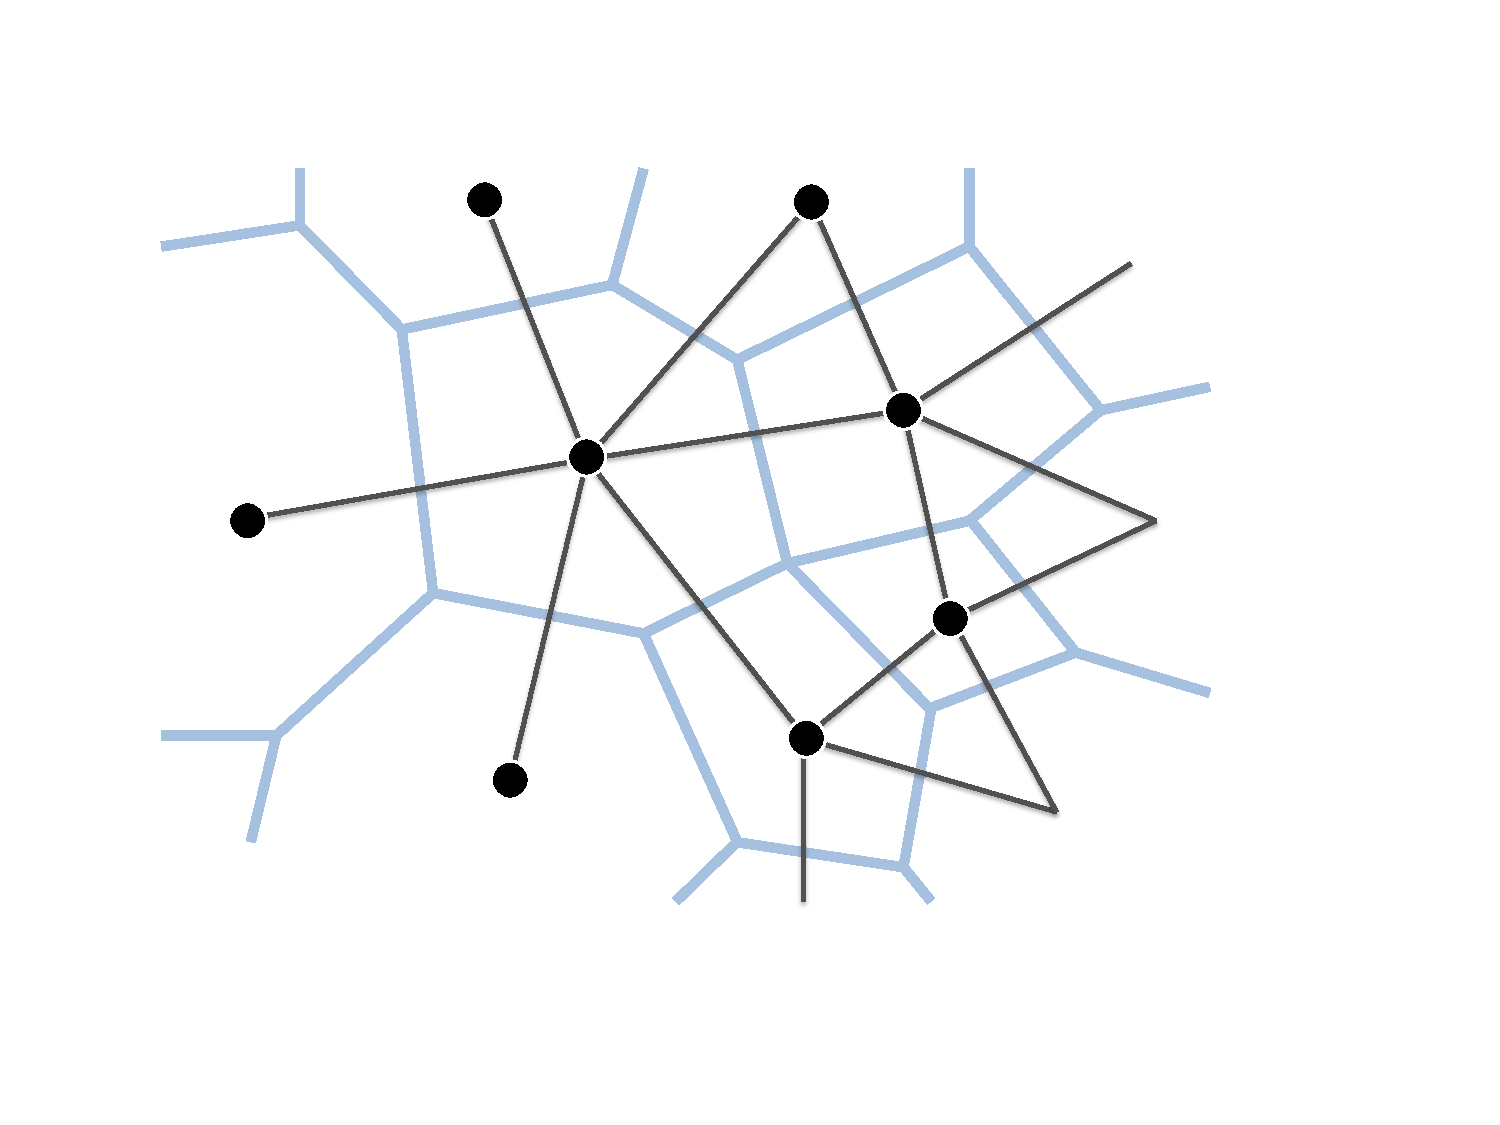
\includegraphics[width=4in]{UnstructuredGrid.pdf}
\end{center}
\caption{An example adjacency graph describing an unstructured grid (blue lines), where nodes are co-located with volume centerpoint locations (solid circles) and edges connect adjacent volumes.} \label{fig:unstructured_grid}
\end{figure}

\begin{figure}[H]
\begin{center}
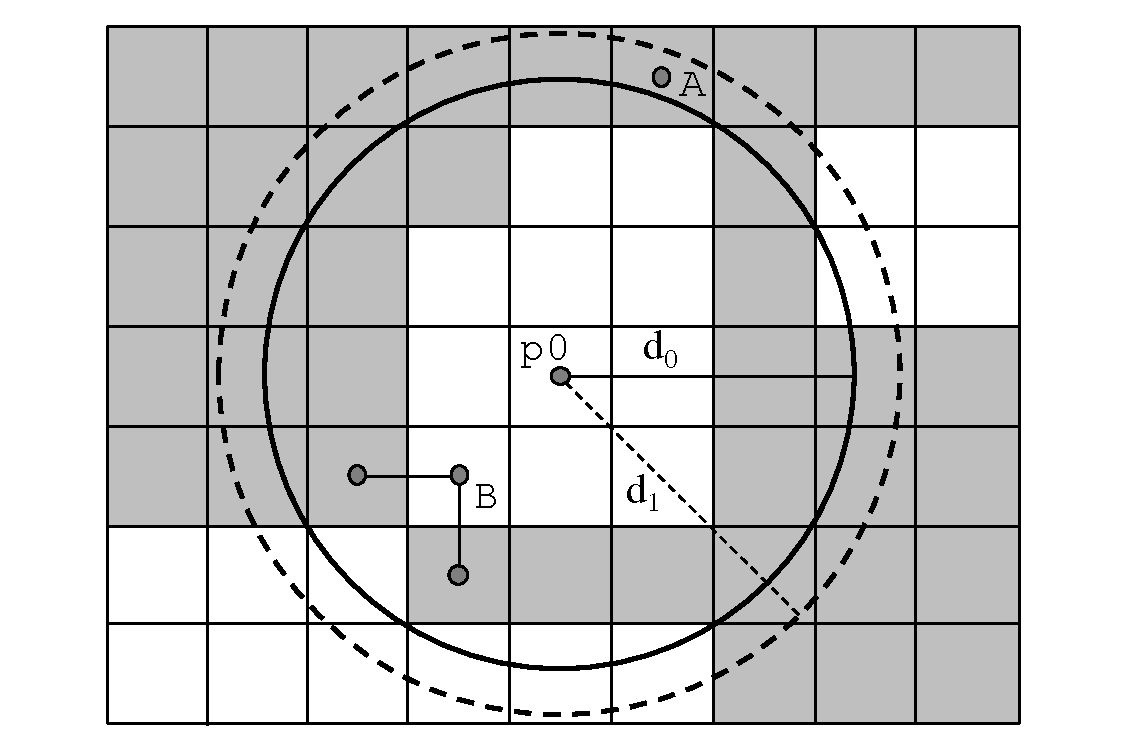
\includegraphics[width=5in]{ClosedContourCriteria2.pdf}
\end{center}
\caption{An illustration of the closed contour criteria.  Nodes shaded in white (gray) satisfy (do not satisfy) the threshold of the field value at \texttt{p0}.  Since only edge-neighbors are included, \texttt{B} constitutes a boundary to the interior of the closed contour.  Because \texttt{A} lays outside the solid circle, the contour with distance $d_0$ is not a closed contour, whereas the dashed contour with distance $d_1$ does satisfy the closed contour criteria.} \label{fig:ClosedContour}
\end{figure}

\begin{figure}[H]
\begin{center}
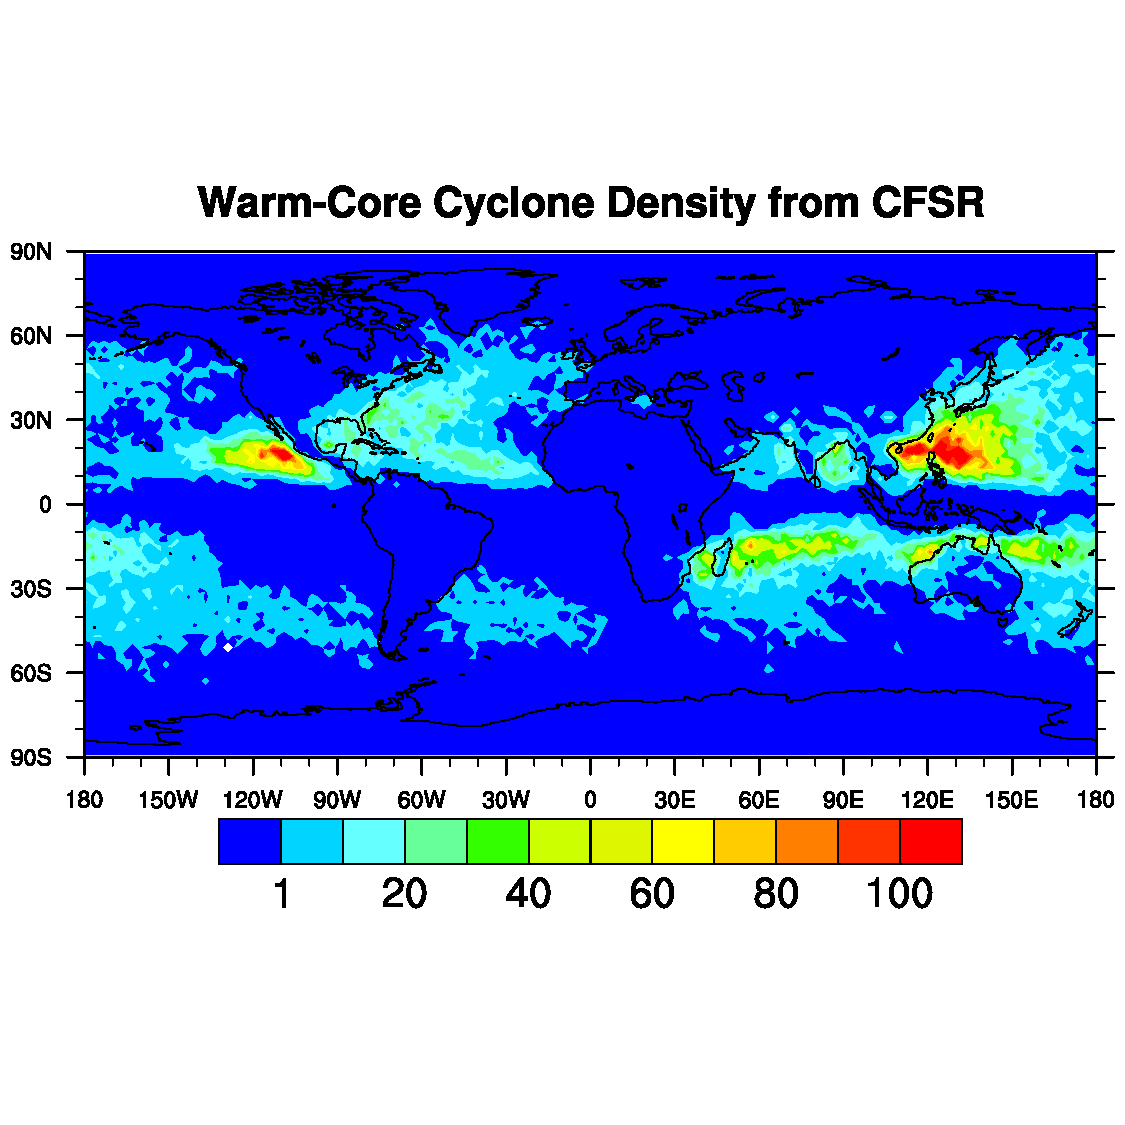
\includegraphics[width=4in, clip, trim=0.2cm 3.6cm 0.2cm 3.1cm]{plot-cfsr_tc_density.pdf}
\end{center}
\caption{Tropical cyclone counts within each $2^\circ \times 2^\circ$ grid cell over the period 1979-2010 obtained using the procedure described in section \ref{sec:TropicalCycloneExample}.} \label{fig:TropicalCycloneDensity}
\end{figure}

\begin{figure}[H]
\begin{center}
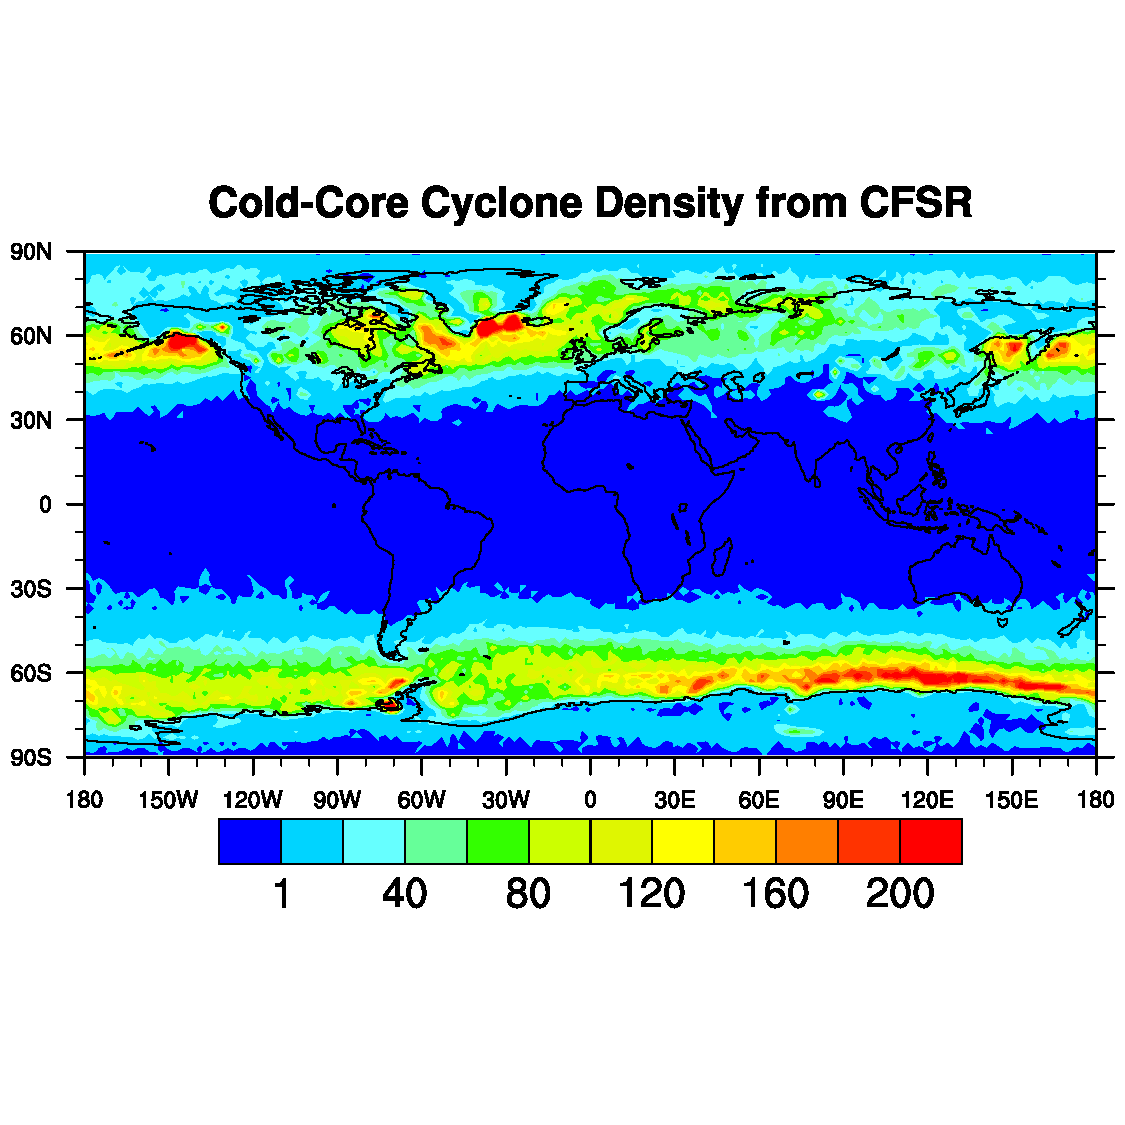
\includegraphics[width=4in, clip, trim=0.2cm 3.6cm 0.2cm 3.1cm]{plot-cfsr_etc_density.pdf}
\end{center}
\caption{Extratropical cyclone counts within each $2^\circ \times 2^\circ$ grid cell over the period 1979-2010 obtained using the procedure described in section \ref{sec:ExtratropicalCycloneExample}.} \label{fig:ExtratropicalCycloneDensity}
\end{figure}

\begin{figure}[H]
\begin{center}
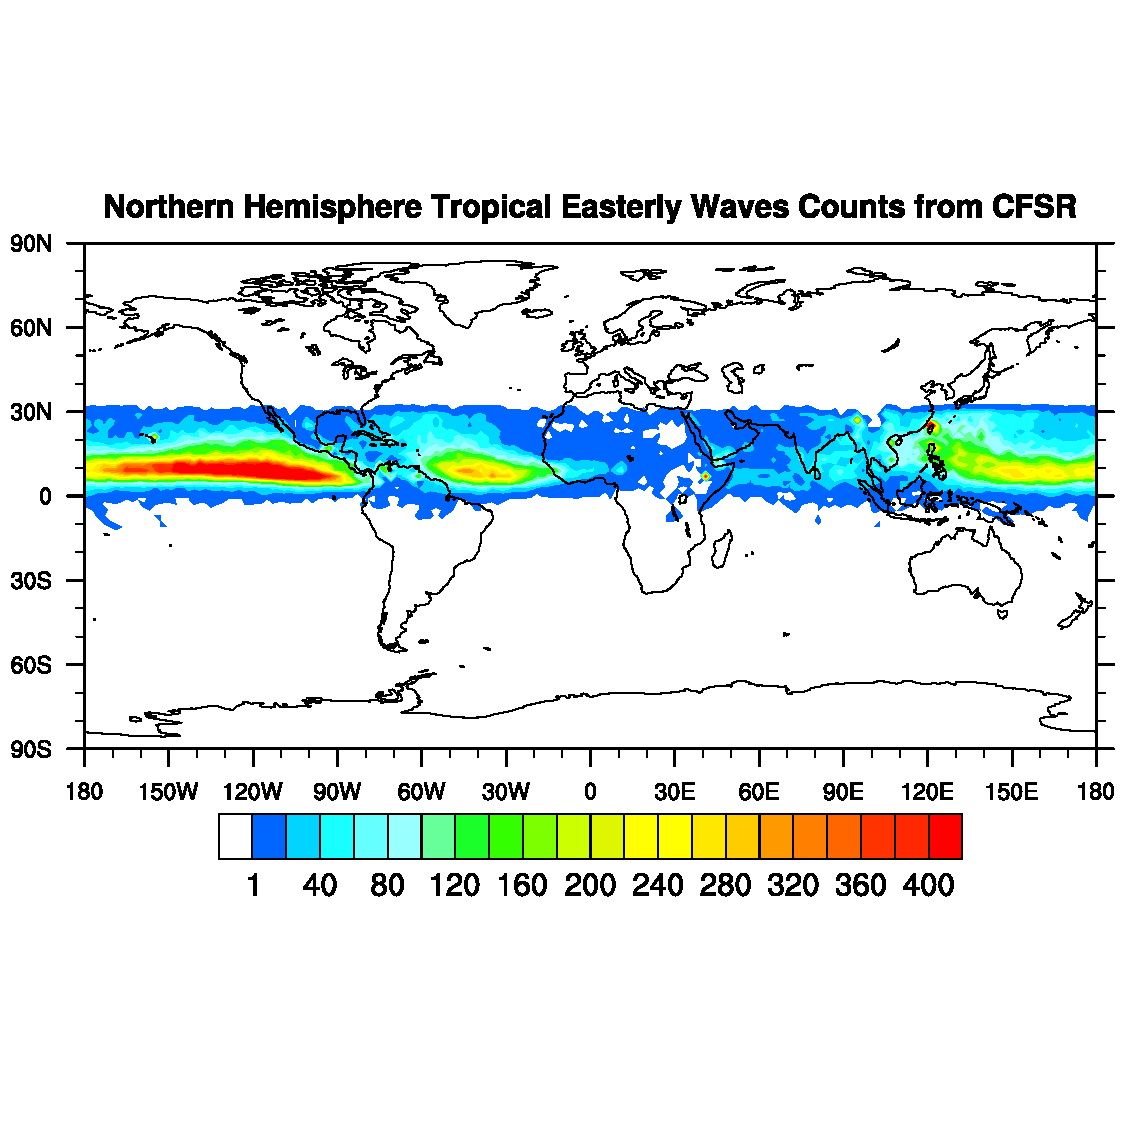
\includegraphics[width=4in, clip, trim=0.2cm 3.6cm 0.2cm 3.1cm]{plot-cfsr_tew_density.pdf}
\end{center}
\caption{Tropical easterly wave counts within each $2^\circ \times 2^\circ$ grid cell over the period 1979-2010 obtained using the procedure described in section \ref{sec:TropicalEasterlyWavesExample}.} \label{fig:TropicalEasterlyWaveDensity}
\end{figure}

\begin{figure}[H]
\begin{center}
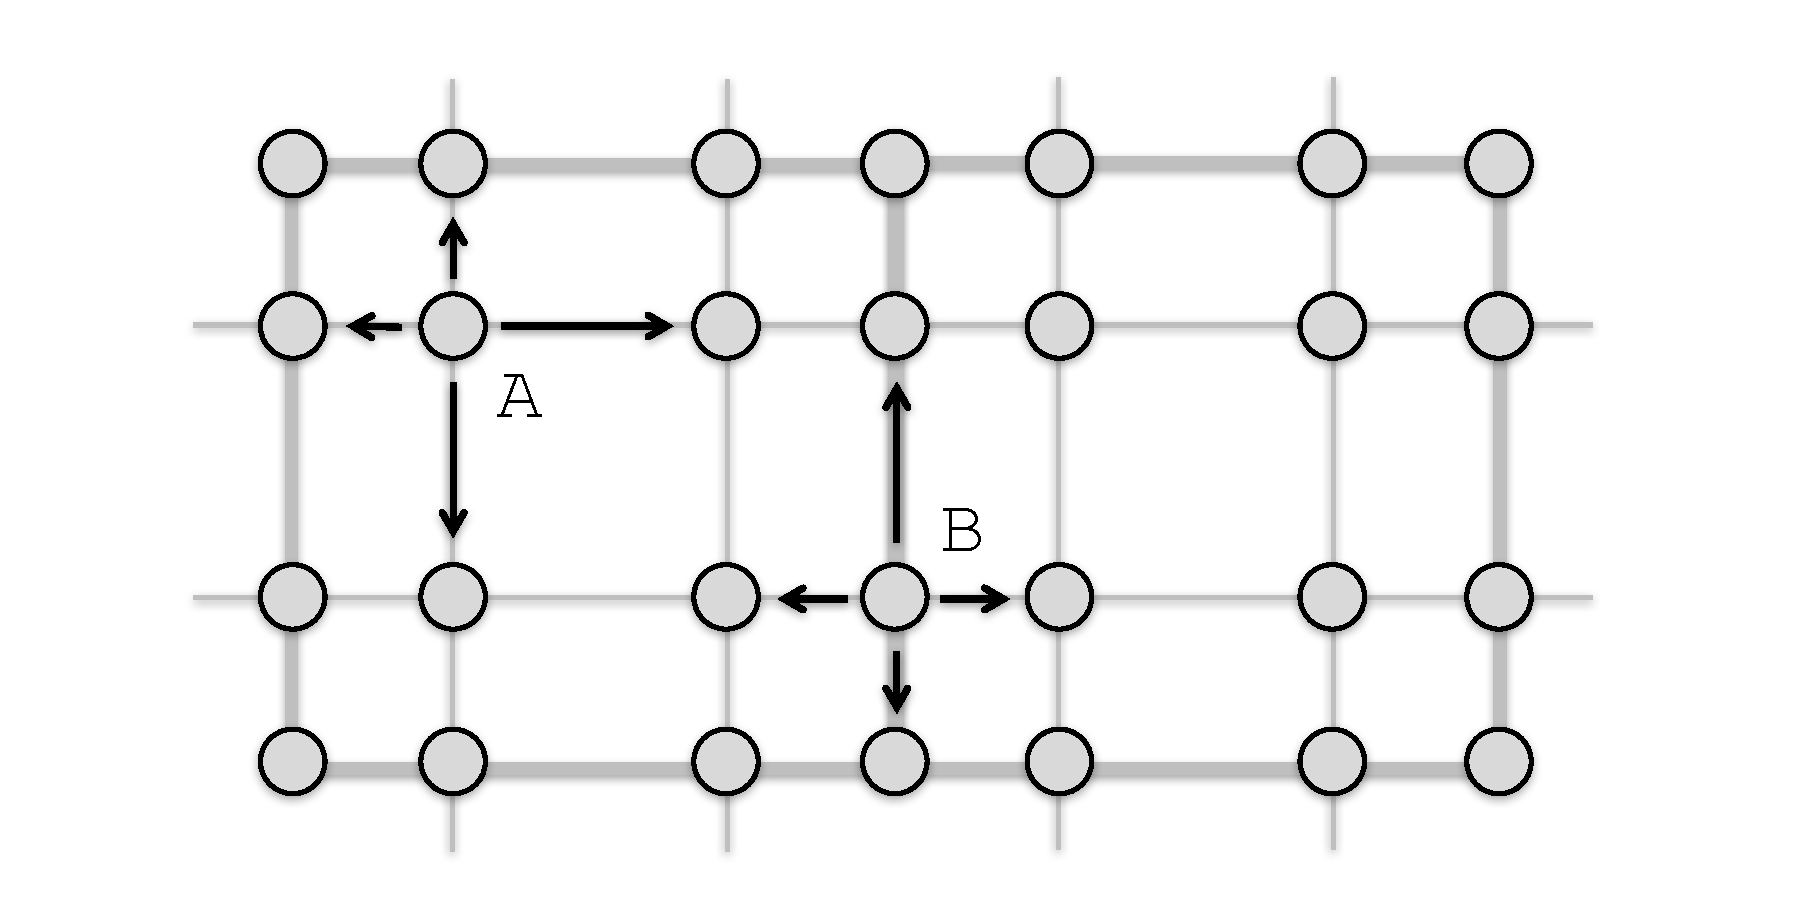
\includegraphics[width=3.5in]{FiniteElementFeatureTracking.pdf}
\end{center}
\caption{An illustration of how connectivity is defined in this work for nodes on a spectral element mesh.  Arrows indicate connectivity for nodes A and B.} \label{fig:FiniteElementConnectivity}
\end{figure}

\begin{figure}[H]
\begin{center}
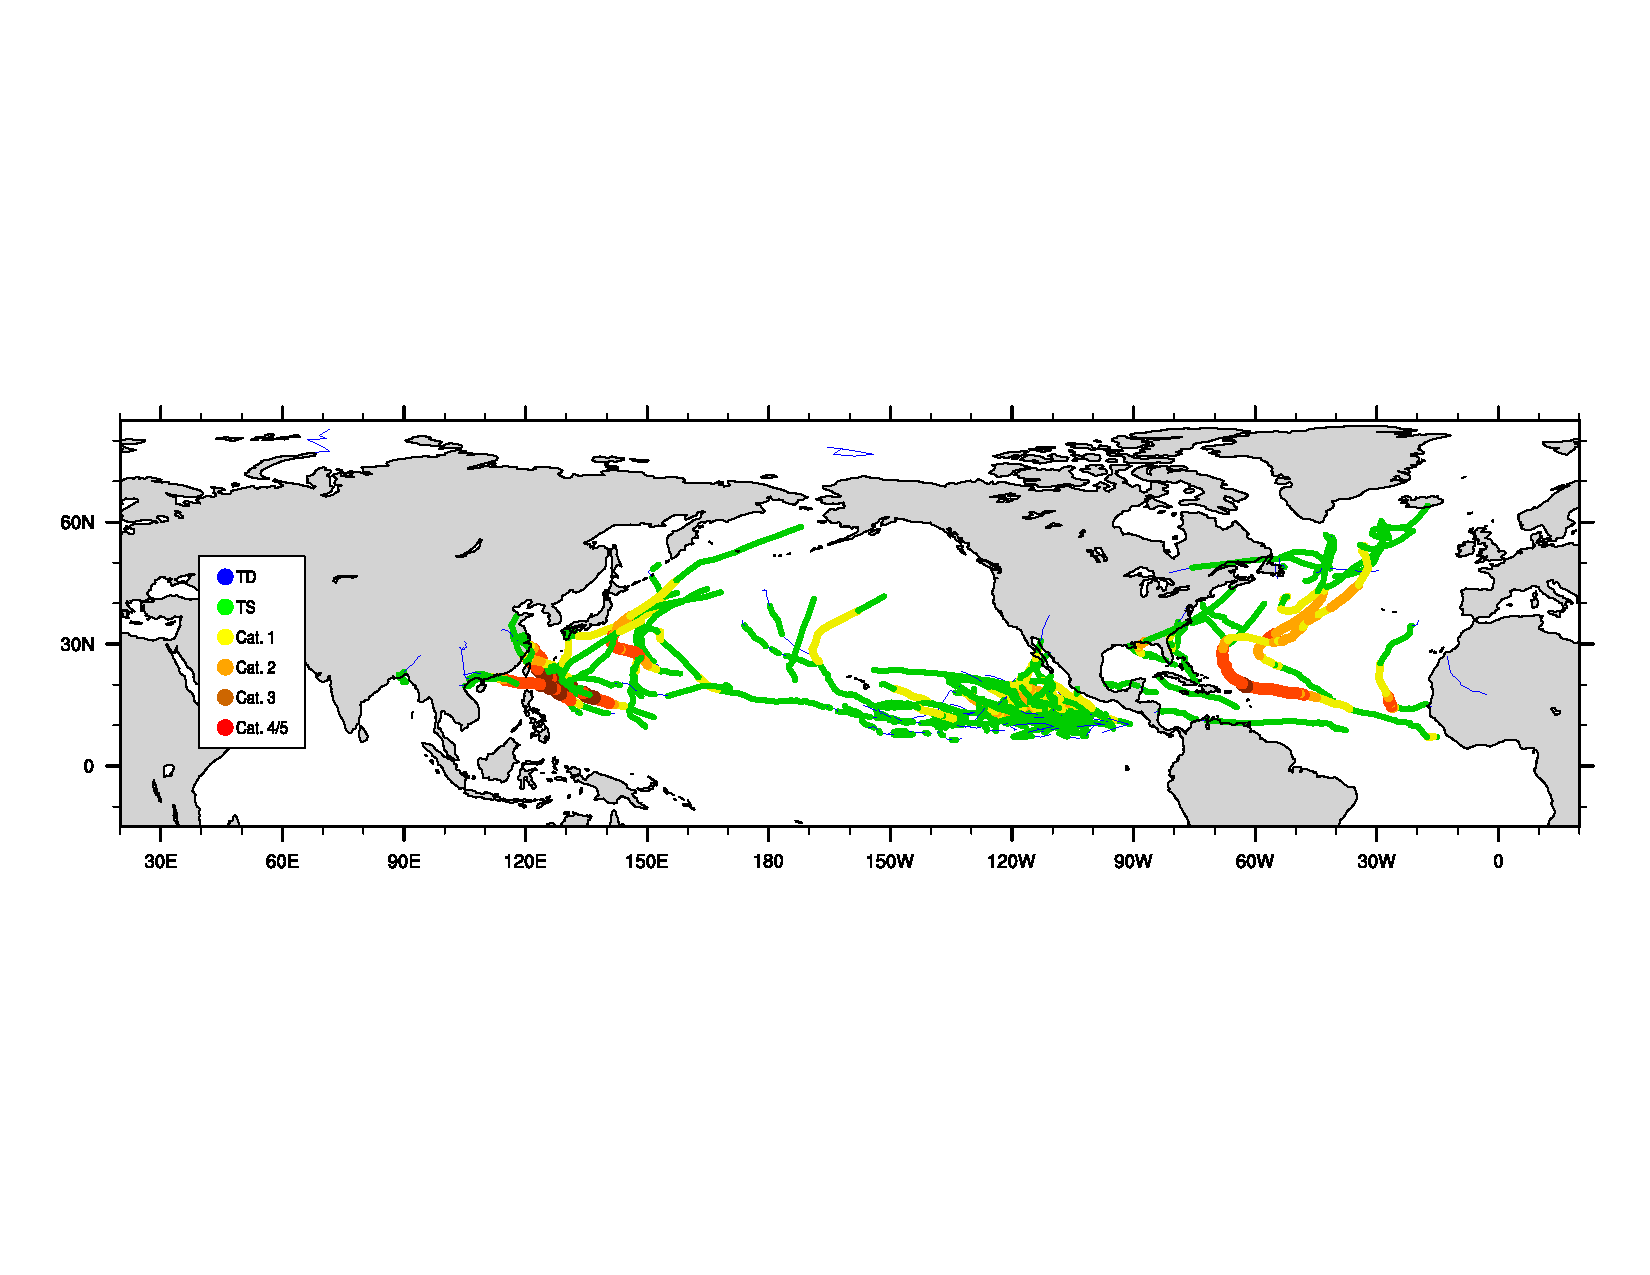
\includegraphics[clip, trim=0.2cm 6.6cm 0.2cm 7.1cm, width=5in]{nhemi-traj_plotted.pdf}
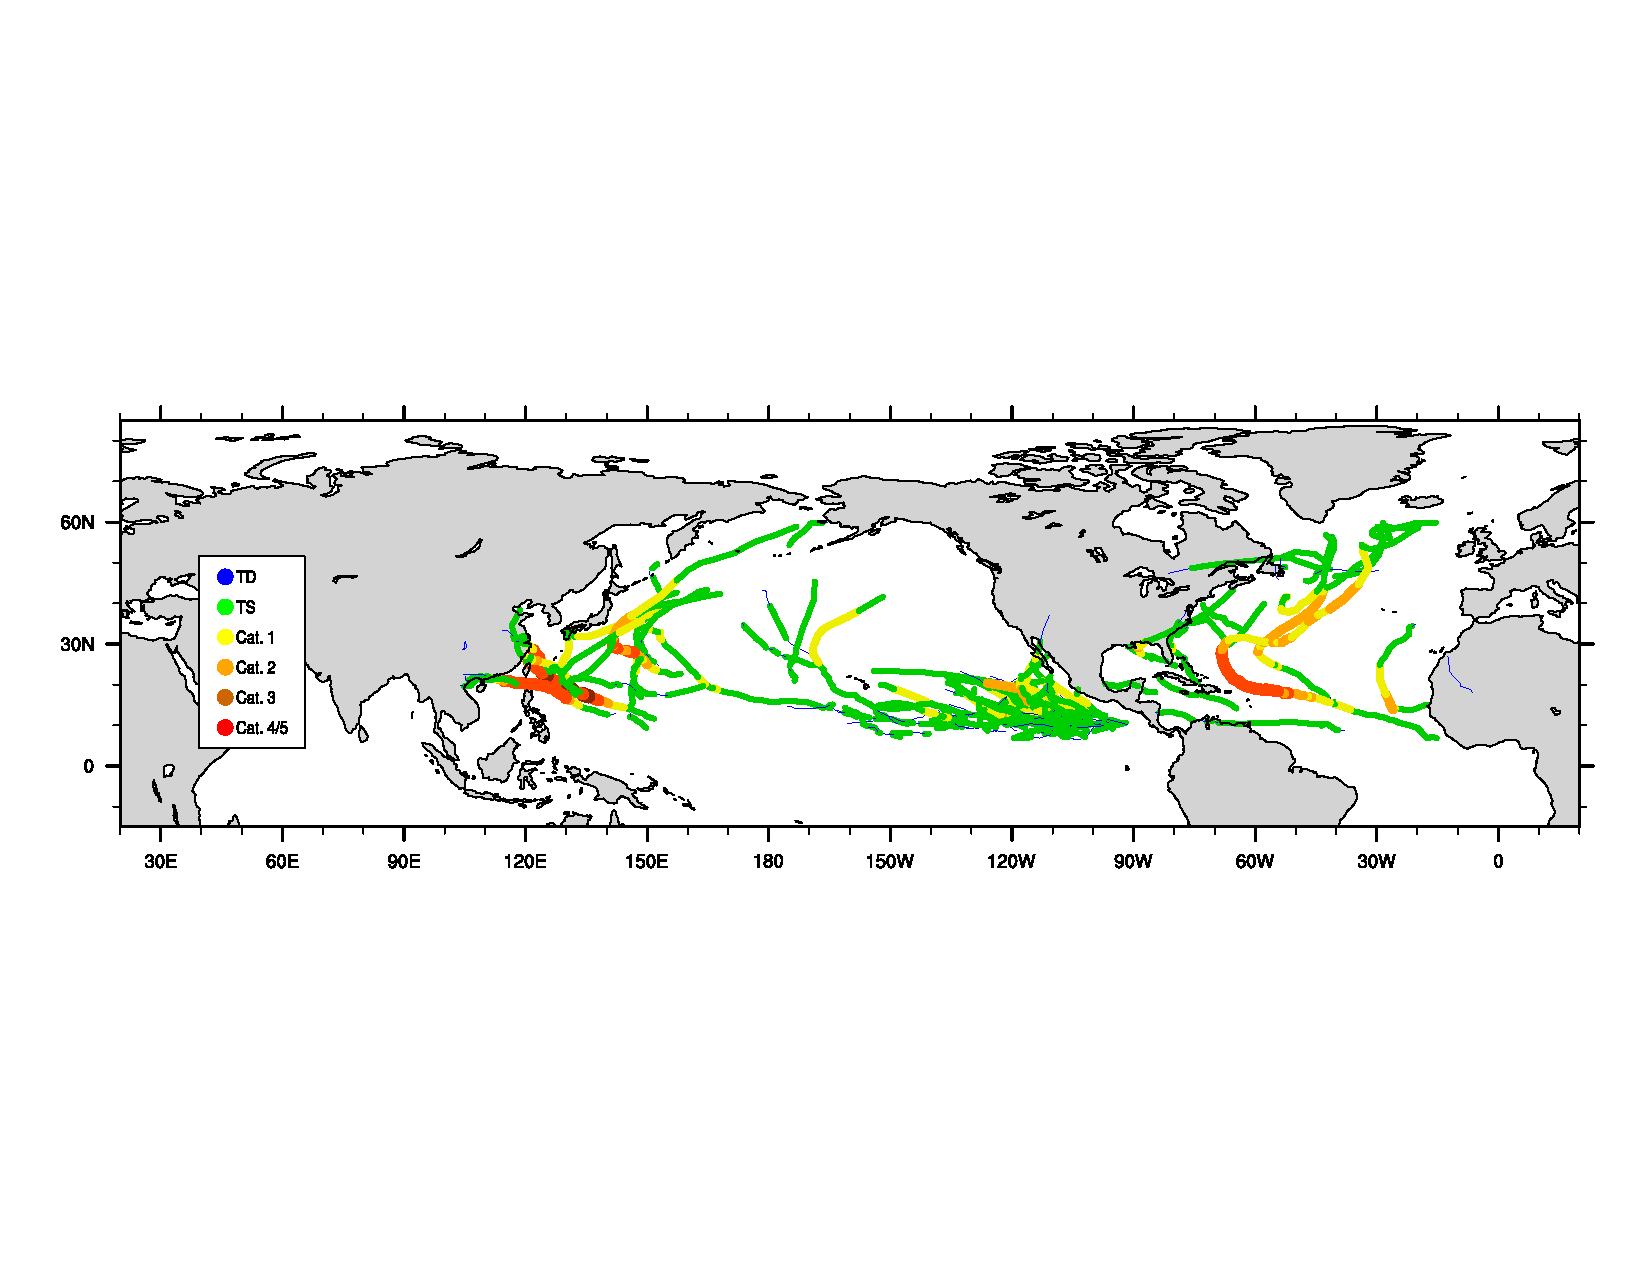
\includegraphics[clip, trim=0.2cm 6.8cm 0.2cm 7.1cm, width=5in]{nhemi_regrid-traj_plotted.pdf}
\end{center}
\caption{Tropical cyclone trajectories and associated intensities as obtained from the simulation of a single hurricane season in CESM \ref{sec:TropicalCycloneCESM} using (top) native spectral-element grid data and (bottom) data regridded to a regular latitude-longitude grid with 0.25$^\circ$ grid spacing.} \label{fig:TropicalCycloneCESM}
\end{figure}

\begin{figure}[H]
\begin{center}
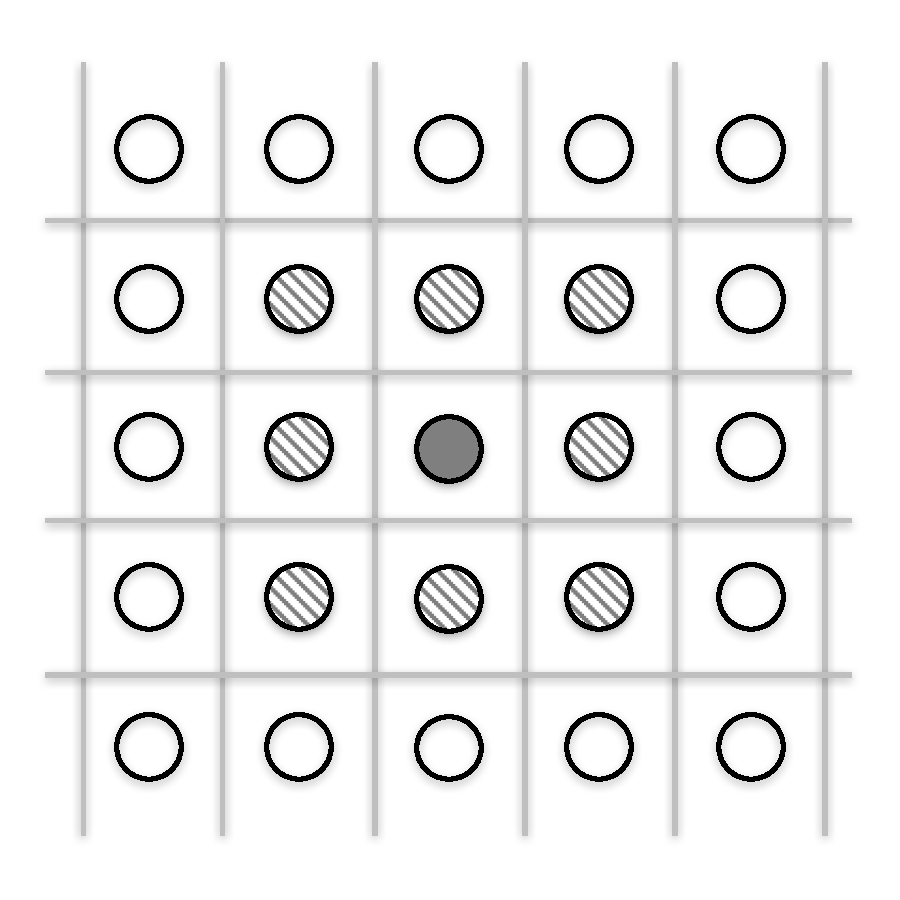
\includegraphics[width=2in]{LocalNodeTypes.pdf}
\end{center}
\caption{The local neighborhood of a central node (shaded) typically refers to the surrounding 8 nodes (diagonal hatching).  The periphery (used by \cite{tsutsui1996simulated}), refers to the set of nodes that surround the local neighborhood (unshaded nodes).} \label{fig:LocalNodeTypes}
\end{figure}


\bibliography{FeatureTrackingBibliography}
\bibliographystyle{copernicus}

\end{document}
